% ===== MARK DISTRIBUTION =====
%  10  Analysis
%  15  Documented Design
%  15  Iterative Development
%  15  Testing
%  15  Evalutation
% =============================

% ========= MY SCORE =========
%  0   Analysis
%  0   Documented Design
%  0   Iterative Development
%  0   Testing
%  0   Evalutation
% =============================

\documentclass{article}
\usepackage{amsmath}
\usepackage{fancyhdr}
\usepackage{listings}
\usepackage{subcaption}
\usepackage{graphicx, float}
\usepackage{multirow, pgfplotstable}
\usepackage{multicol}
\usepackage{pythonhighlight}
\usepackage{color}
\usepackage{bookmark}
\usepackage[a4paper, total={150mm, 210mm}, margin=60pt]{geometry}
\usepackage{hyperref}
\hypersetup{
    colorlinks=true,       % Use colored text instead of boxes
    linkcolor=black,        % Color for internal links (e.g., TOC entries)
    urlcolor=cyan,         % Color for URLs
    citecolor=green,       % Color for citations (optional)
    filecolor=magenta      % Color for file links (optional)
}
%command for creating spaces
\newcommand\tab[1][0.5cm]{\hspace*{#1}}

\newcommand{\mr}[3]{\multirow{#1}{#2}{#3}}
\title{\textbf{NEA}}
\author{Name: Jez Snelson\\
        Candidate Number: 1209\\
        Centre Number: 62337}
%Footer and Header
\fancyhead[L]{Computer Science NEA}
\fancyhead[R]{Oxford Spires Academy, Center No. 62337}
\fancyfoot[L]{Jez Snelson, Candidate No. 1209}
%Margins
\setlength{\marginparwidth}{0pt}
\pgfplotsset{compat=1.18}
\begin{document}
\pagenumbering{roman}
\date{}
\pagestyle{empty}
\maketitle
\newpage
\tableofcontents
\newpage
\pagestyle{fancy}
\pagenumbering{arabic}
\section{Analysis}
        \subsection{Dungeon Crawlers}
        A dungeon crawl is a scenario in role playing games in which the main character navigates a dungeon environment often solving traps or fighting monsters to progress through the level. A video game or board game made up of predominantly dungeon crawls is considered to be a dungeon crawler.\\
        \\
        Most dungeon crawlers have a fixed map that is the same every time which can lead to little replay value as it can be boring to replay the same map over and over.\\
        \subsection{The Problem}
        Dungeon Crawler style games can be boring and repetitive, this means they can have little to none replay value. Additionaly alot of Dungeon crawlers have a steep learning curve that makes it hard for new or casual players to fully enjoy them. These games are also very complex often demanding lots of time for a simple playthrough. In addition, Non-Computational Methods are inconvenient as they can take up alot of space, take a long time to set up and you cannot save your game state to pick it up later easily.\\
        \subsection{Stakeholders}
        \subsubsection{Survey}
        I chose a set of questions in order to survey my stakeholders and help me find success criteria for the project to fulfill their needs.\\
        1. How often would you say you play video games on a scale of 1-10 (1 being every other week 10 being every day)\\
        2. Do you have any specific or requirements for this computer game?\\
        3. How would you use this game?\\
        4. Would you say you have the time to commit to learning a complex or unintuitive game?(yes,probably not,no)\\
        5. How long would you say is your average gaming session?(1-5 hours)\\
        6. Which different ways do you play video games?(multiple choice: controller, wasd, arrows)\\
        7. Have you played any Dungeon Crawler games(e.g. Legend of Zelda, Binding of Isaac, Dead Cells, Hades)?\\
        8. If not would you want to try a Dungeon Crawler Game?\\
        9. Rank the features of classic dungeon crawlers you dislike the most(Lack of Replayability, Long Unskippable Cinematics, High length of time required for a playing session, The Learning Curve, The Difficulty)\\
        10. Rank the features you think are most essential for the game to be enjoyable for you(Procedurally Generated Dungeons, Loot to Collect and utilise, Some Sort of skill tree, Co-Op mode, Puzzles, Hidden Areas)\\
        \newpage
        \subsubsection{Survey Results}
        Time available:\\
        On average my stakeholders session length is around 2 hours for a single game. On average they play videogames almost every day however there is one that plays infrequently. Because of this I will have to try and make it easy to pick up without much you have to remember about previous sessions.\\
        Most of my stakeholders do not have time to commit to learning a complex or unintuitive game and so I will have to make the game easy to pick up but still have complexities for those who want a challenge.\\
        All controlling mechanisms where popular but WASD was the most so I will prioritise that.\\
        50\% of my stakeholders have played dungeon crawlers and so may be experienced with it but 50\% have not so I should aim to make it a good introduction to the dungeon crawler genre with the potential of adding optional difficulty for those more experienced.\\
        \\
        Disliked Features (Ranked most to least disliked):\\
        1. Lack of replayability.\\
        2. High length of time required for a playing session.\\
        3. The Learning Curve.\\
        4. Long Unskippable Cinematics.\\
        5. The Difficulty.\\
        Due to this I will focus on replayability through the use of procedural generation whilst still aiming to exclude the more disliked features.\\
        \\
        Liked Features (Ranked from most to least liked):\\
        1. Some sort of skill tree.\\
        2. Hidden Areas\\
        3. Procedurally Generated Dungeons.\\
        4. Loot to collect and utilise (e.g. weapons).\\
        5. Puzzles.\\
        6. Co-Op Mode.\\
        Because of this I will prioritise getting the more liked features done and exclude some of the less liked features from my success criteria.\\
        \subsubsection{About Stakeholders}
        \begin{tabular}{|c|c|c|}
                \hline
                Name & Description & How they will use my product\\
                \hline
                \mr{2}{3cm}{Samuel Vanderstelt-Hook} & \mr{2}{6cm}{18 year old Male Sixth Form Computer Science Student, Casual Gamer who enjoys a wide range of games.} & \mr{2}{5cm}{Sam will use my solution for casual gaming for fun as a break from his studies. He has stated needs for a game that is replayable and gives him a reason to come back to it.}\\
                &&\\
                &&\\
                &&\\
                &&\\
                &&\\
                \hline
                \mr{2}{3cm}{Daniel Olde Scheper} & \mr{2}{6cm}{18 year old Male A Level Computer Science Student} & \mr{2}{5cm}{Daniel will use my solution as a way to relax from his A-Level Studies. He has stated needs for a fun, replayable and easy to pick up game.}\\
                &&\\
                &&\\
                &&\\
                &&\\
                \hline
                \mr{2}{3cm}{Peter Dunn} & \mr{2}{6cm}{17 year old Male College Student and aspiring hobbyist game developer.}& \mr{2}{5cm}{Peter will use my solution as a form of entertainment after studies and as he loves Dungeon Crawl Style games. He needs a replayable game with an intuitive combat system.}\\
                &&\\
                &&\\
                &&\\
                &&\\
                &&\\
                \hline
                \mr{2}{3cm}{Sadiya Shorkar} & \mr{2}{6cm}{17 year old Female Student and Casual Video Game Enjoyer} & \mr{2}{5cm}{Sadiya will use my solution as a form of  casual entertainment for short sessions. Sadiya has seizures and so needs accessibility options like volume control and options for less vibrancy.}\\
                &&\\
                &&\\
                &&\\
                &&\\
                &&\\
                &&\\
                \hline
                \mr{2}{3cm}{Penelope Castiau} & \mr{2}{6cm}{18 year old Female Sixth Form Student, Avid Computer Gaming Enjoyer and Hobbyist Streamer.} & \mr{2}{5cm}{Penny will use my product for entertainment purposes and to play on stream. Because of this Penny needs subtitles to make the game easy to follow for viewers.}\\
                &&\\
                &&\\
                &&\\
                &&\\
                &&\\
                \hline
                \mr{2}{3cm}{Steff Stylianos} & \mr{2}{6cm}{17 year old Female College Student and Game Developer} & \mr{2}{5cm}{Steff will use my product to relax from studies. Steff needs a replayable game but also want it to be engaging.}\\
                &&\\
                &&\\
                &&\\
                \hline
        \end{tabular}
        \newpage
        \subsection{Research}
        \subsubsection{Existing Solutions}
        \textbf{Edmund McMillen's The Binding of Isaac}\\
        Edmund McMillen created the popular dungeon crawler roguelike The Binding of Isaac and released it on Steam$_{(1)}$.
        This game was relatively unique as it had procedurally generated dungeons \\using a system of rooms that tesalate with each other.\\
        \\
        The procedurally generated dungeons consist of different shaped square based rooms that tesalate and are generated next to each other in a psuedo random fashion whilst obeying a set of rules. The mobs that spawn in each room can vary but there is usually only one or two enemy types per room and as you go up levels the amount of enemies and difficulty the pose increases. This system allows for every playthrough of the game to be different to the next with the same reccuring theme/difficulty which allows for lots of replay oppurtunity. This would be an appropiate way for me to fix the replayabilty issue.\\
        \\
        I like the games simple UI design as it clearly indicates all the necessary parts. The Map also shows the basic stucture of the level without revealing too much. I want to take inspiration from the simplicity of ui in order to help my game be intuitive.\\
        \\
        However, the game has a couple issues that mean that it does not completely solve our problem. First is the steep learning curve that the game presents which, although to some is a welcome challenge, can put off new or less experienced players especially due to its roguelike nature meaning when you die you start from scratch. The game also has an unintuitive movement and fighting system as there is only really quad directional projectiles and a simple walking design which when combined contributes to the steep learning curve. These are some of the features I will not include in my product opting to instead try for an easier approach by allowing scaleable difficulty and oct-directional movement and attacks.\\
        \begin{figure}[h]
                \centering
                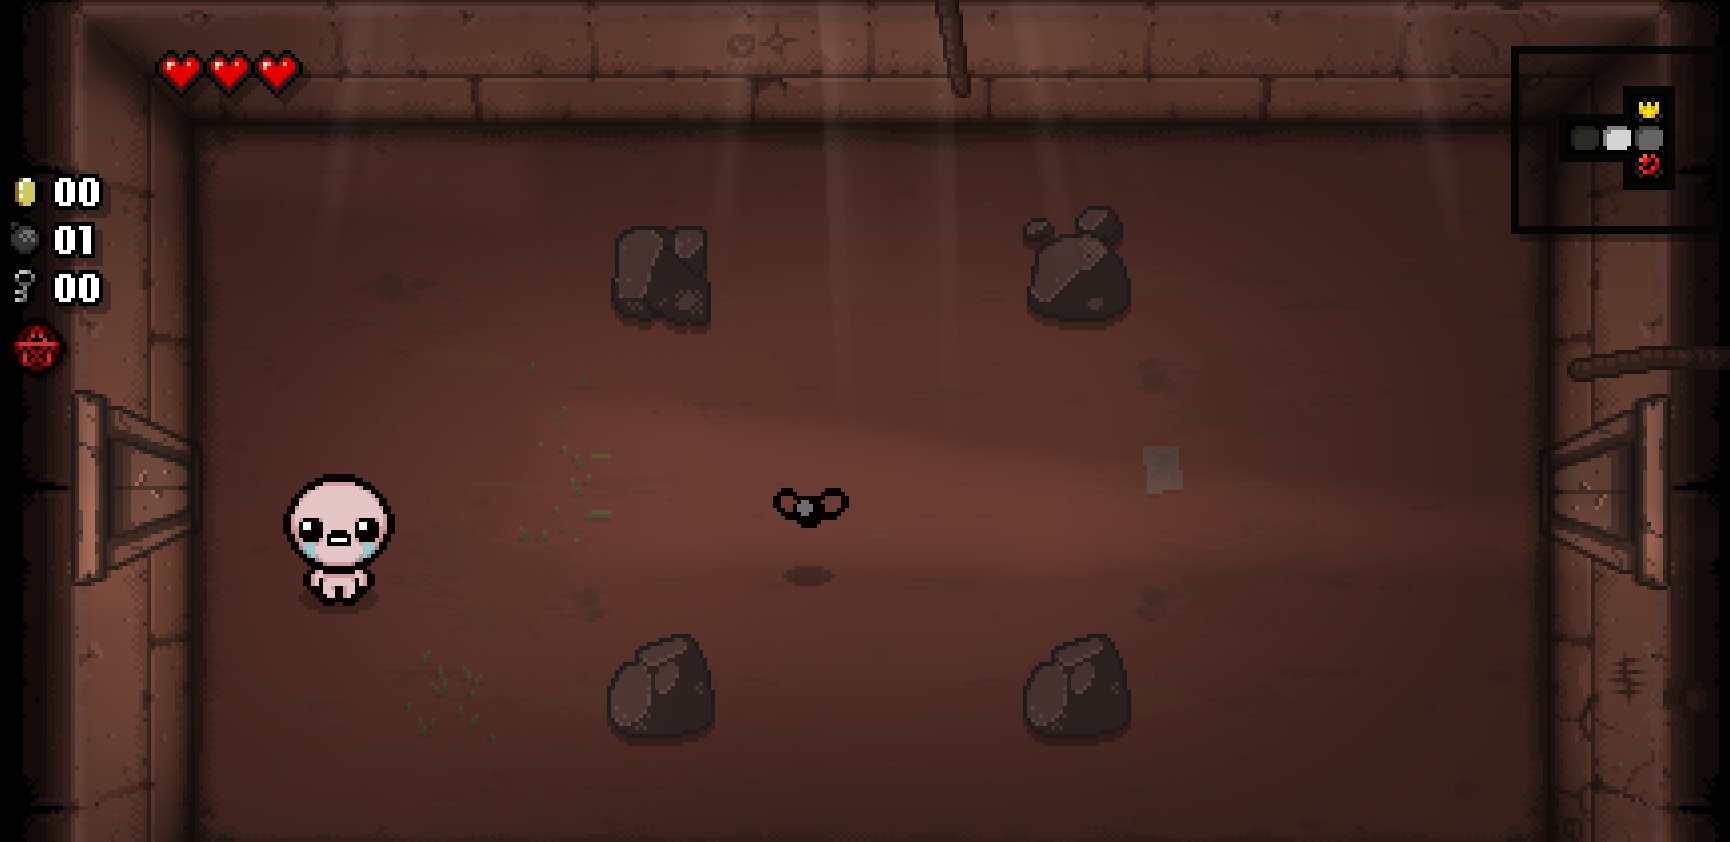
\includegraphics[scale=0.25]{images/research/BOI_Capture.PNG}
                \caption{A screenshot of The Binding of Isaac UI and Map}
        \end{figure}
        \newpage
        \[\]
        \textbf{Motion Twin's Dead Cells}\\
        Motion Twin created the roguelike dungeon crawler and metroidvania Dead Cells which is released on steam$_{(2)}$. This game is known for its permadeath system and its procedurally generated dungeons.\\
        \\
        The way Dead Cells uses procedural generation interests me as it allows for there to be some fixed attributes to the level whilst still allowing elements of randomness. The developers talk about how they do this in a video devlog$_{(3)}$, here the dev talks about his system of having a fixed structure for each level almost like a skeleton. This skeleton will include stuff like important rooms along the way and how much distance of rooms has to be between them. It then fills in all the spaces for rooms with one of the many handmade rooms made by the developers. After one room has been chosen for a spot this leaves less choice for the other spots as the rooms need to join and flow into each other properly and so as it chooses more of them the structure of the level is determined similar to the wave function collapse algorithm$_{(4)}$.\\
        \\
        This style of generation allows for a unique experience each time whilst keeping a hand crafted and natural feel to the levels that is often lost in other techniques. Because of these advantages I will take heavy inspiration from this style of procedural generation for my level generation in order to make them more unique.\\
        \\
        However due to the game being aimed at more hardcore gamers with it being part of the rouguelike genre it can often appear complex and offputting to newer players who dont like the idea of taking multiple runs just to have very little to show for it and not much forward progress in the game. Although the game is a side on game I think that I will use the idea of its procedural generation as inspiration in my product aswell as aiming to forgo some of the games more complex or challenging mechanics such as permadeath in order to create a more accessible game.\\
        \begin{figure}[H]
                \centering
                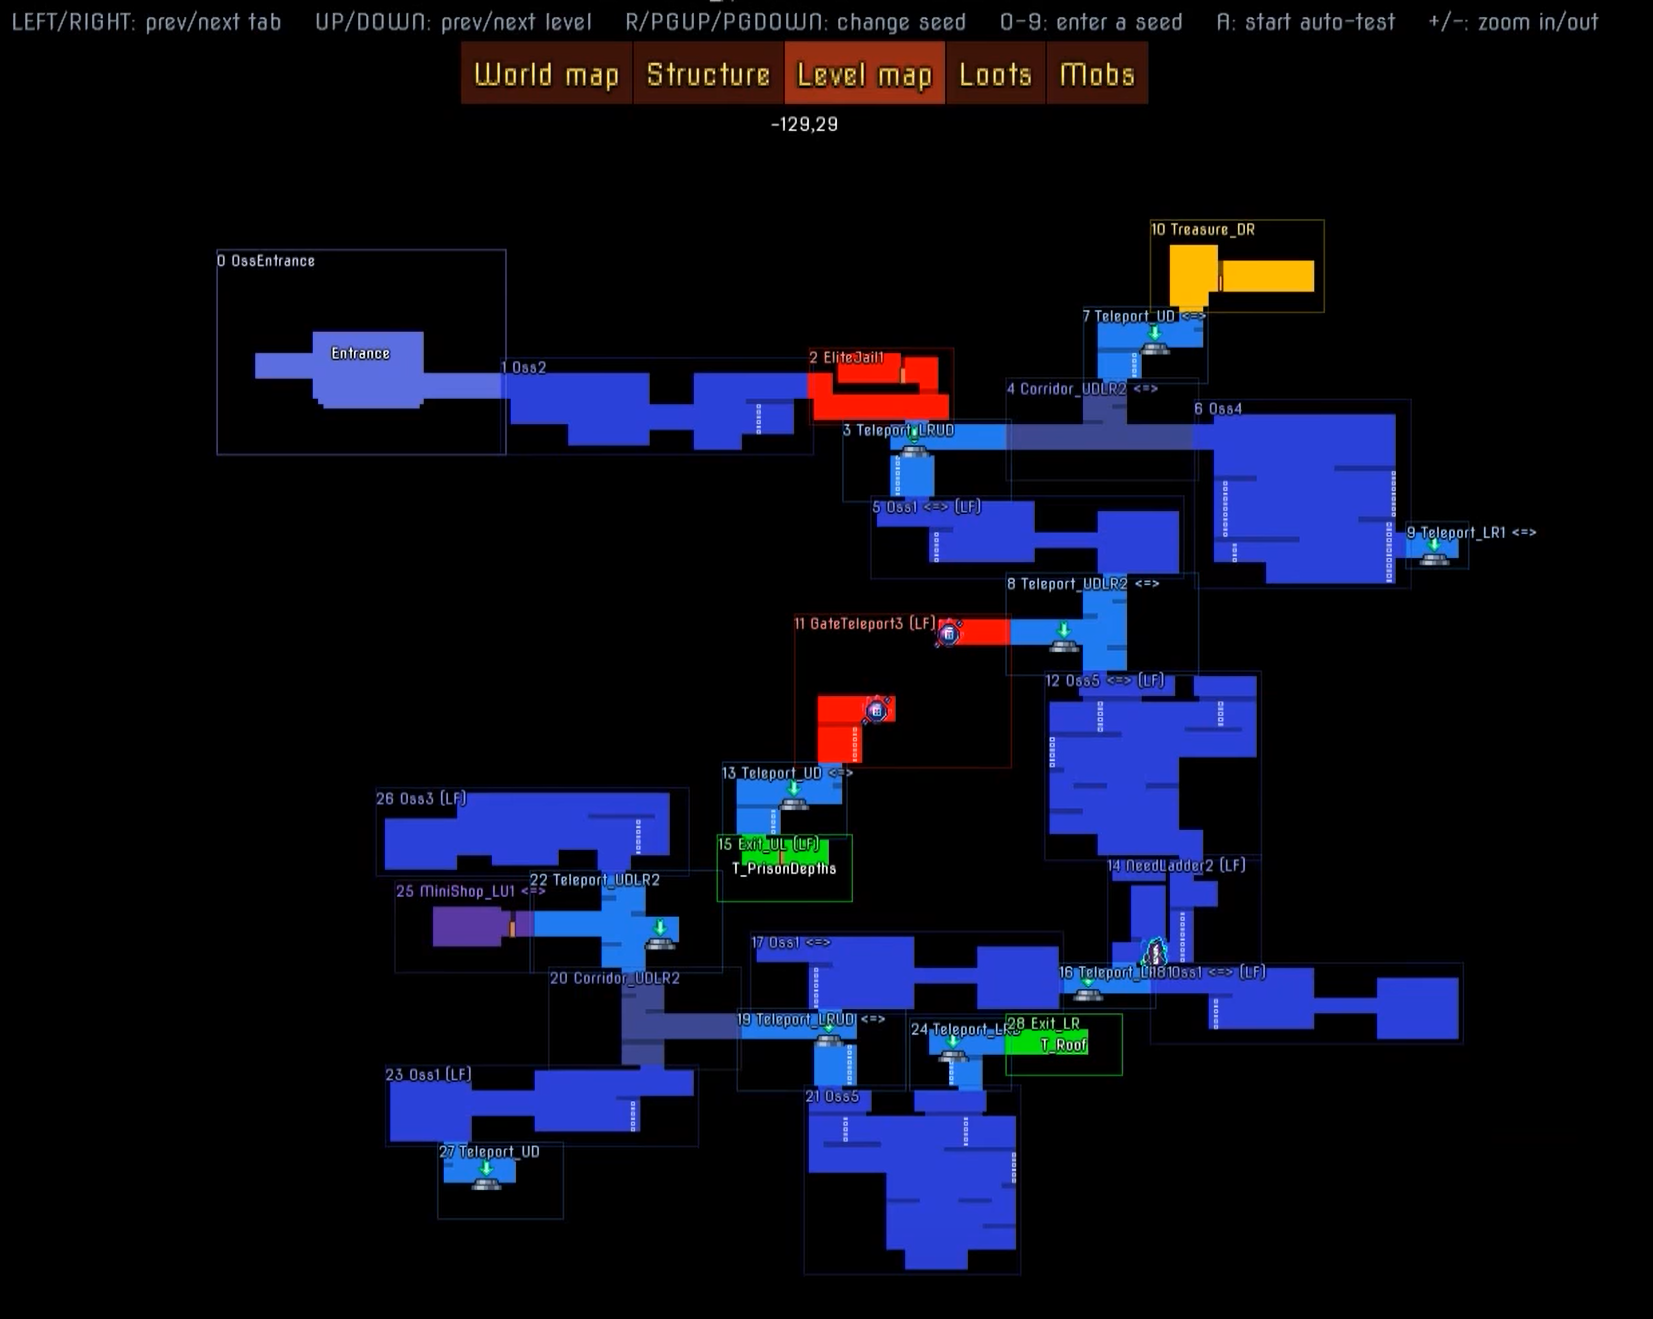
\includegraphics[width = 0.8\columnwidth]{images/research/Dead_Cells_level_gen.PNG}
                \caption{Dead Cells Level Generation Example}
        \end{figure}
        \newpage
        \[\]
        \textbf{Nintendo's Legend Of Zelda Breath of the Wild}\\
        Nintendo created the open-world dungeon crawler which is released on the Nintendo Wii U and the Nintendo Switch$_{(5)}$. This game is known for its open world approach to dungeon crawlers as well as its easy to pick up nature for first time players.\\
        \\
        The game starts with a tutorial that teaches players the mechanics of the game (combat, exploration, and resource gathering). This tutorial helps players into the world without overwhelming them, offering opportunities to learn at their own pace which helps reduce the steep learning curve of other games in the genre. The open-world nature of the game also adds to its replayability, allowing the player to take many different routes to complete the game. However, while the game’s size and allows for alot of replayabilty, the volume of content and time required to explore everything can reduce its effectiveness as a game that can be picked up easily for shorter sessions. Its 3D world and complex systems are features that would be too tricky to implement within the scope of an A-level computer science project. It also does not fully fit the dungeon-crawler genre, particularly as it is less dungeon-focused.\\ 
        \\
        I want to take inspiration from the open-world nature of the game to allow different routes through my game to increase replayability aswell as its approach to tutorials in order to make the learning curve steeper. Ontop of this another feature I would like to take inspiration from is the intuitiveness of the combat system which is easy to learn but hard to master in particular its feature of being able to lock onto enemies.\\
        \\
        Some features I will not be including are the 3D nature and the overall content heaviness aswell as the focus less on dungeon crawling as I believe these would be unnecesary features which would drive up the complexity of the solution both to make and run.\\
        \begin{figure}[H]
                \centering
                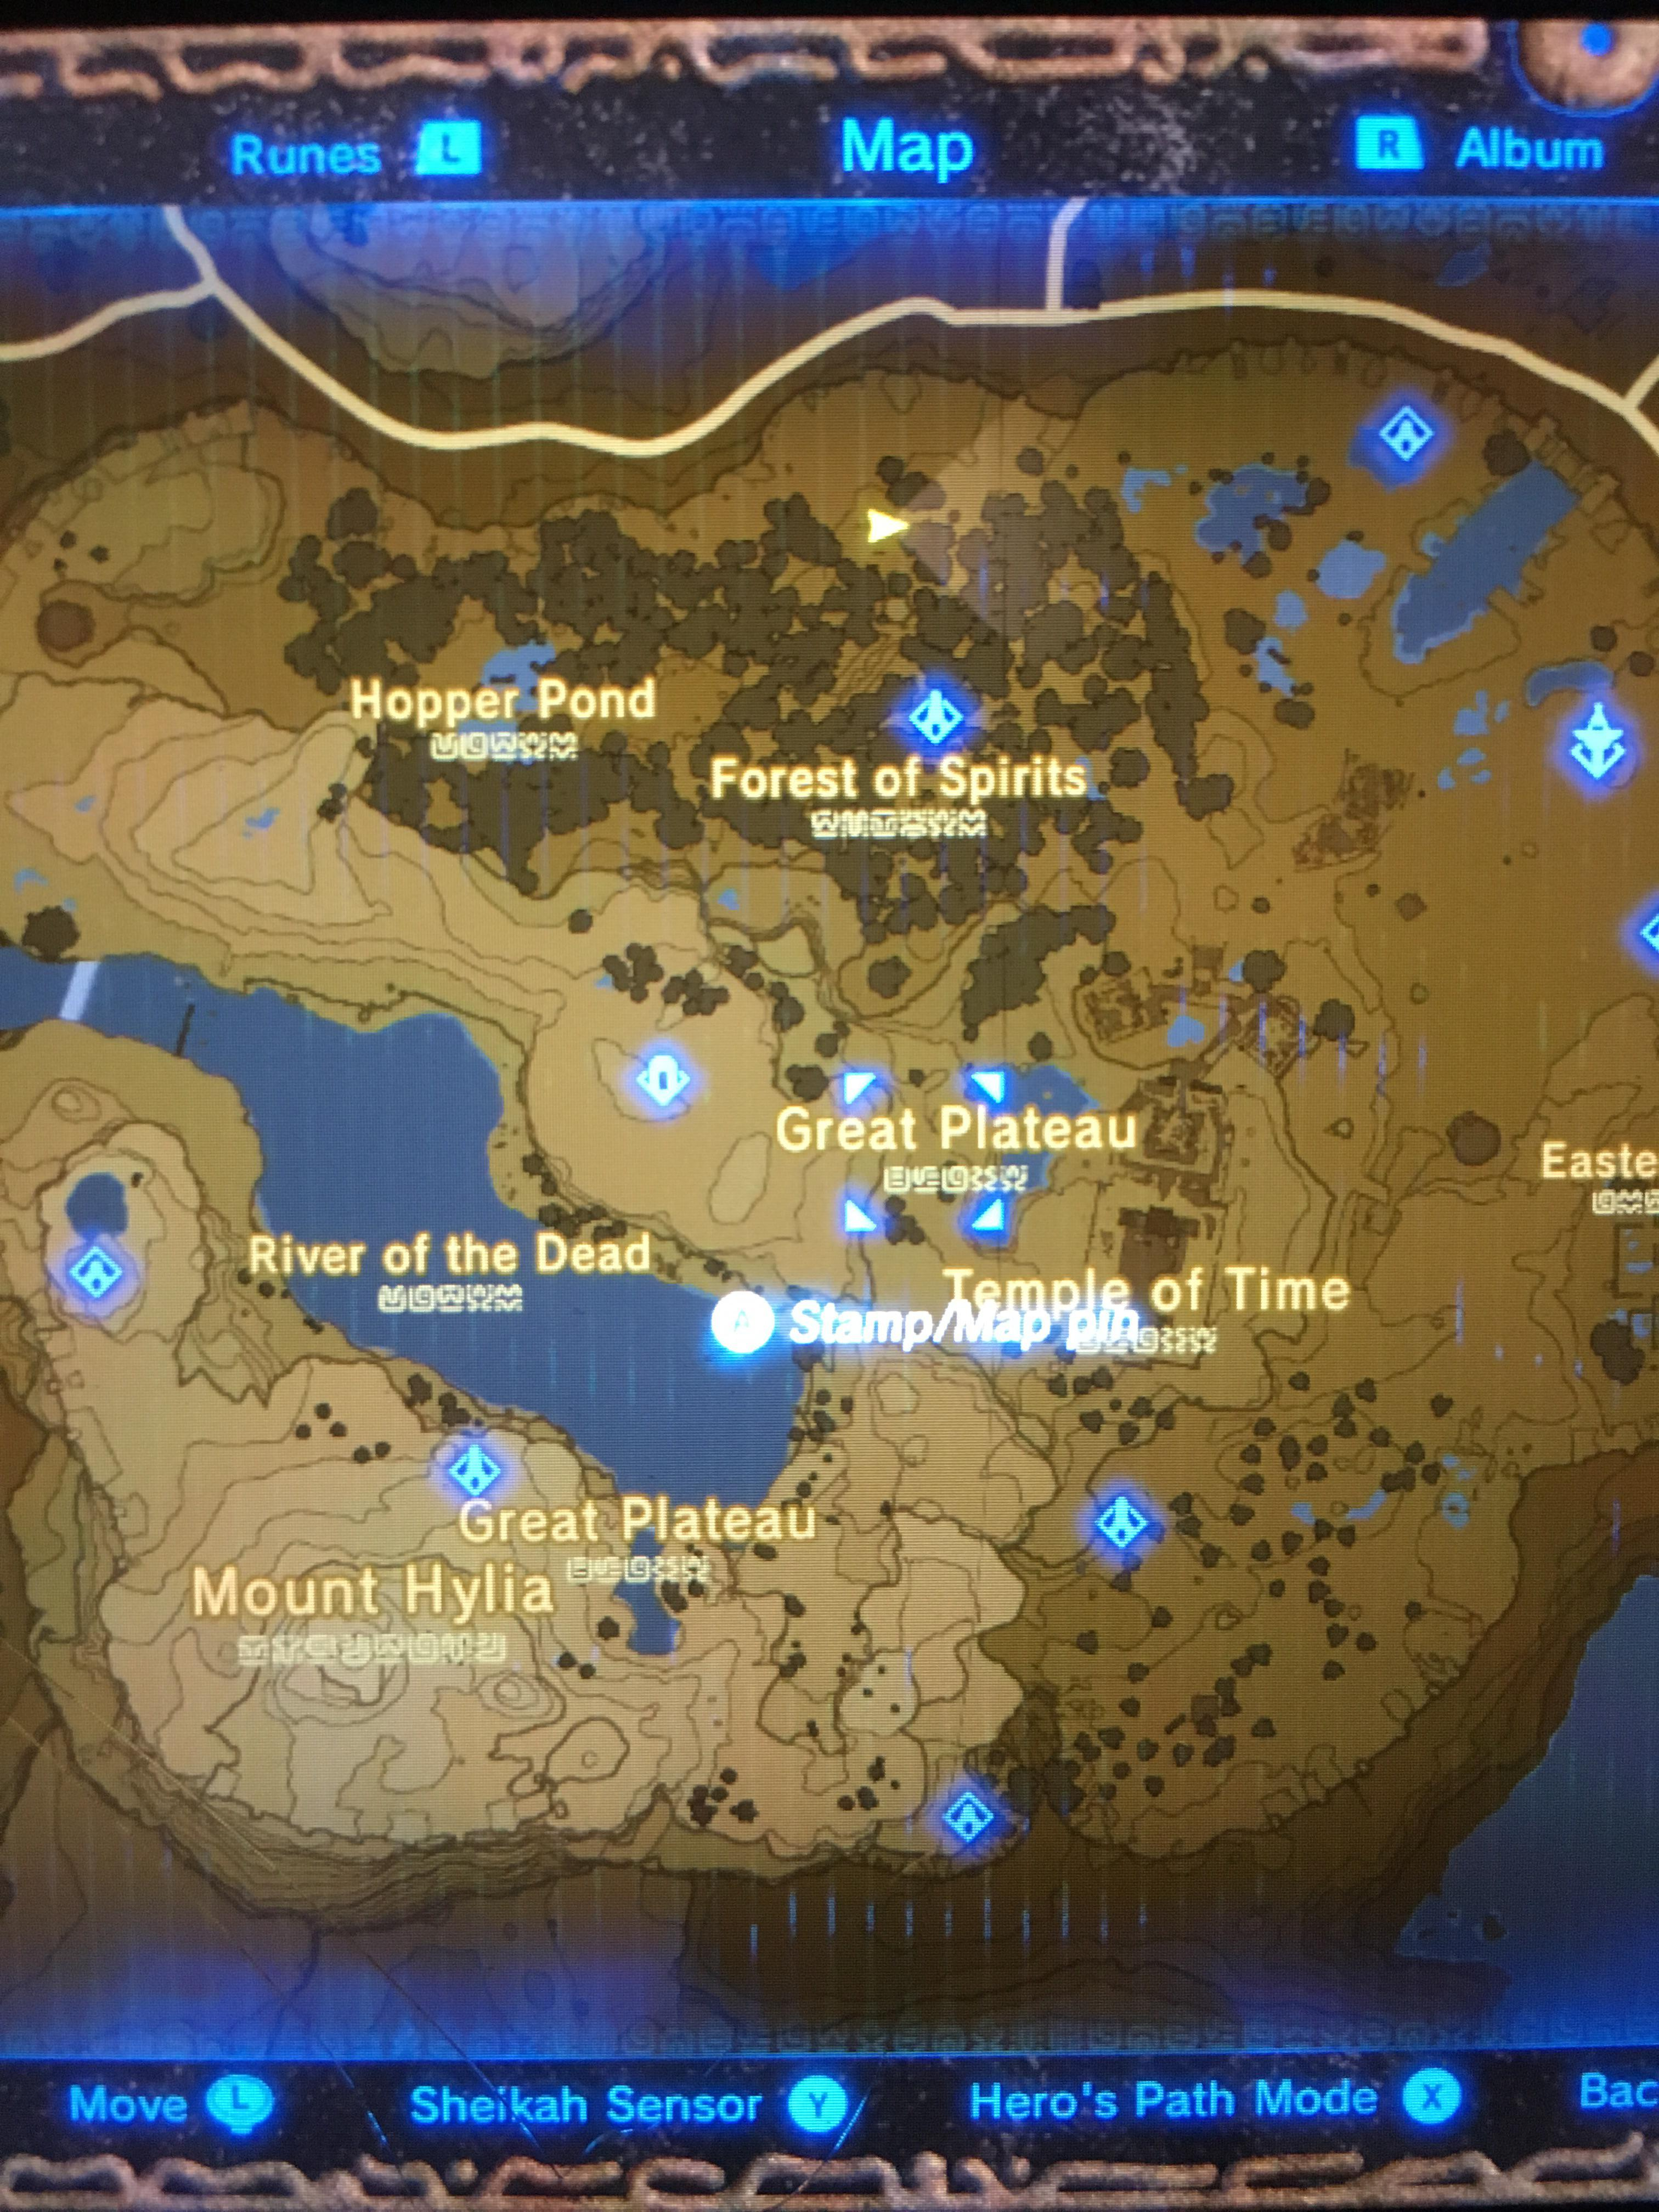
\includegraphics[width = 0.5\columnwidth]{images/research/BOTW_tutorial_map.jpg}
                \caption{BOTW tutorial map}
        \end{figure}
        \noindent This map shows how the BOTW tutorial has the different "shrines" placed to help the player learn the basic mechanics of the game.\\
        \newpage
        \[\]   
        \subsection{Limitations and Requirements}
        \begin{tabular}{|c|c|c|}
                \hline
                Requirement&Description&Justification\\
                \hline
                \mr{2}{3cm}{Hardware}&\mr{3}{7cm}{PC or laptop with a Keyboard or Game Controller, minimum of 4GB RAM.\\For Windows/Linux: x86\_32 CPU with SSE2 instructions, any x86\_64 CPU, ARMv8 CPU.\\For Macos: x86\_64 or ARM CPU.\\Integrated graphics with full OpenGL 3.3 support}&\mr{3}{5cm}{These are the requirements for running an executable from Godot. The keyboard(WASD) or controller is needed as the input for the game.}\\
                &&\\
                &&\\
                &&\\
                &&\\
                &&\\
                &&\\
                &&\\
                &&\\
                \hline
                \mr{2}{3cm}{Software}&\mr{2}{7cm}{I will be using the Godot Game Engine and GDScript to program my game.}&\mr{3}{5cm}{I will be using Godot as it is a good 2D game designer that is Free and Open-Source it changes less often than alternatives such as Unity. Ontop of this I have prior experience in Godot and GDScript.}\\
                &&\\
                &&\\
                &&\\
                &&\\
                &&\\
                &&\\
                &&\\
                \hline
                \mr{2}{3cm}{OS Limitations}&\mr{3}{7cm}{For Native Exports:  Windows 7 or newer, macOS 10.13 or newer, Linux distribution released after 2016\\For Web: Firefox 79, Chrome 68, Edge 79, Safari 15.2, Opera 64}&\mr{3}{5cm}{Godot can export easily to any of these platforms and more accessibility is good and I can also export a HTML5 version to be hosted in a website such as https://www.itch.io.}\\
                &&\\
                &&\\
                &&\\
                &&\\
                &&\\
                \hline
                \mr{2}{3cm}{General System Limitations}&\mr{3}{7cm}{A visually or auditory excellent experience}&\mr{3}{5cm}{I do not have the experience with shaders or music and sound effects to add these features to the game in this time and it would make the game requirements higher.}\\
                &&\\
                &&\\
                &&\\
                &&\\
                &&\\
                \hline
        \end{tabular}
        \subsection{Features}
        \subsubsection{Essential Features}
        \begin{tabular}{|c|c|c|c|}
                \hline
                Feature\#&Feature&Description&Justification\\
                \hline
                1&\mr{2}{3cm}{Player Movement and Controls}&\mr{2}{5cm}{The player will control movement using the WASD keys for up, left, down and right respectively Q will trigger a dash. Alternatively they will use the left control stick of a controller.}&\mr{2}{5cm}{This will be used to navigate around the Dungeon environment and WASD was the most popular control mechanism for the stakeholders with controller close behind. The controls of my game aim to follow the stakeholder feedback aswell as the general controls that seemed to be favoured in my research}\\
                &&&\\
                &&&\\
                &&&\\
                &&&\\
                &&&\\
                &&&\\
                &&&\\
                &&&\\
                &&&\\
                &&&\\
                \hline
                2&\mr{2}{3cm}{A Basic Combat System}&\mr{2}{5cm}{The combat system will consist of a primary weapon (melee, magic or ranged) on mouse-1/1 key/X button and a sheild or secondary weapon on mouse-2/2 key/Y button. I will have to implement projectiles and hitboxes for both the player and enemies.}&\mr{2}{5cm}{A basic combat system is essential as it will provide the main difficulty and entertainment within the game. The existing solutions all have at least a basic combat system as one of the driving forces for progress through the game.}\\
                &&&\\
                &&&\\
                &&&\\
                &&&\\
                &&&\\
                &&&\\
                &&&\\
                &&&\\
                \hline
                3&\mr{2}{3cm}{Dungeon Environment}&\mr{2}{5cm}{The Dungeon Environment will consist of different shaped rooms with different purposes(e.g. boss room, chest room and shop room.) with hallways connecting inbetween them and a starting room.}&\mr{2}{5cm}{A Dungeon Environment is essential as it is the environment the player will play in. All the existing solutions had dungeon environments as this is an essential part of a 'dungeon crawler'.}\\
                &&&\\
                &&&\\
                &&&\\
                &&&\\
                &&&\\
                &&&\\
                \hline
                4&\mr{2}{3cm}{Different Enemies}&\mr{2}{5cm}{The Enemies will consist of a variety of enemies that attack the player with different patterns and have different looks and animations.}&\mr{2}{5cm}{This is essential as it will add variety to the gameplay and each enemy will provide a challenge to the player as I saw it used during my research.}\\\
                &&&\\
                &&&\\
                &&&\\
                &&&\\
                \hline
                5&\mr{2}{3cm}{Appearance and Animations of the Player}&\mr{2}{5cm}{The Player will have a recognisable appearance aswell as animations for all its actions such as walking and fighting}&\mr{2}{5cm}{This is essential as it tells you about where your character is aswell as what they are doing even if the animations are basic like in Binding of Isaac.}\\\
                &&&\\
                &&&\\
                &&&\\
                &&&\\
                \hline
                6&\mr{2}{3cm}{Login System}&\mr{2}{5cm}{Users will be able to login in order to save and reload their progress. The login system will use a username and password with the details being encrypted and stored in an external database. Their will be options for signing in or creating a new account aswell as resetting your password.}&\mr{2}{5cm}{This is an essential feature as saving progress is essential for making the game replayable. All the Exisiting solutions I looked at either had login systems or used an existing login system (e.g. steam) in order to manage seperate user saves.}\\
                &&&\\
                &&&\\
                &&&\\
                &&&\\
                &&&\\
                &&&\\
                &&&\\
                &&&\\
                &&&\\
                \hline
                7&\mr{2}{3cm}{User Interface}&\mr{2}{5cm}{A Simple UI that shows status indicators like health, weapons being used, enemy health and magic points.}&\mr{2}{5cm}{This would allow the player to be aware of the characters health and communicate necessary information for playing the game as I found through the Binding of Isaac UI.}\\
                &&&\\
                &&&\\
                &&&\\
                &&&\\
                &&&\\
                \hline
        \end{tabular}
        \subsubsection{Desireable Features}
        \begin{tabular}{|c|c|c|c|}
                \hline
                Feature\#&Feature&Description&Justification\\
                \hline
                8&\mr{2}{3cm}{Weapons and a more Advanced Combat System.}&\mr{2}{5cm}{A system of weapons where you can get them from boss drops and potentially shops and a combat system with normal, charged (based on how long you hold down) and special attacks (using a special key).}&\mr{2}{5cm}{Different weapons will allow each player to have a playstyle more customized to them and will allow for the player getting stronger as they progress more. An advanced combat system will allow for a more smooth and enjoyable fighting experience as I saw through my research into Dead Cells and BOTW.}\\
                &&&\\
                &&&\\
                &&&\\
                &&&\\
                &&&\\
                &&&\\
                &&&\\
                &&&\\
                &&&\\
                &&&\\
                \hline
                9&\mr{2}{3cm}{Skill Tree}&\mr{2}{5cm}{A skill tree to unlock unique skills/abilities and get better at using existing skills/weapons. You would gain points from playing the game and can then put them into different areas in order to create a customized character build}&\mr{2}{5cm}{This would further allow the player to choose their own play style and add an element of replayability where you can try going for a different build each time you play. This was also requested by the stakeholders and can be seen in Dead Cells.}\\
                &&&\\
                &&&\\
                &&&\\
                &&&\\
                &&&\\
                &&&\\
                &&&\\
                \hline
                10&\mr{2}{3cm}{Procedurally Generated Dungeons}&\mr{2}{5cm}{The Dungeons would be procedurally generated whilst keeping some amount of structure (e.g. the same amount of distance between posses and key rooms). This would happen through many similar small room sections that can be slotted together in order to make a full dungeon.}&\mr{2}{5cm}{This would create a more engaging game which is different each time you play it and therefore increase replayability exponentially as the different combinations of room increases. This was also requested by the stakeholders and was used in Dead Cells to allow for greater replayability.}\\
                &&&\\
                &&&\\
                &&&\\
                &&&\\
                &&&\\
                &&&\\
                &&&\\
                &&&\\
                &&&\\
                \hline
                11&\mr{2}{3cm}{Hidden Areas}&\mr{2}{5cm}{Secret areas that can be unlocked through wasy such as progressing further in the game and coming back or through puzzles/fake walls. Could have secret loot or bosses.}&\mr{2}{5cm}{This feature was highly requested by the stakeholders and can be seen in alot of existing solutions and would allow for more time spent having fun in the game through finding these areas.}\\
                &&&\\
                &&&\\
                &&&\\
                &&&\\
                &&&\\
                &&&\\
                \hline
                12&\mr{2}{3cm}{Inventory System}&\mr{2}{5cm}{An Inventory to be opened with the E key or the + button through which you will manage equipped weapons, key items, skills and more.}&\mr{2}{5cm}{An Inventory System is an essential feature if we want to add more weapons/weapon types and a skill tree. It can be seen in BOTW and less complex in Dead Cells.}\\
                &&&\\
                &&&\\
                &&&\\
                &&&\\
                &&&\\
                \hline
                13&\mr{2}{3cm}{Settings and Volume Control}&\mr{2}{5cm}{A settings page to control the volume of noises aswell as the vibrancy of colours.}&\mr{2}{5cm}{One of the Stakeholders has requested this as a feature to help the game be more accessible to them.}\\
                &&&\\
                &&&\\
                &&&\\
                \hline
                14&\mr{2}{3cm}{Difficulty Levels and Hardcore Mode}&\mr{2}{5cm}{A Difficulty level selector which allows the user to up the difficulty(damage the enemies do etc) and a Hardcore Mode which switches the game to a roguelike format with seperate save state to the normal game.}&\mr{2}{5cm}{50\% of the stakeholders are experienced with Dungeon Crawlers so in order to help the game still be reasonably challening for them I will add a difficulty slider.}\\
                &&&\\
                &&&\\
                &&&\\
                &&&\\
                &&&\\
                &&&\\
                \hline
        \end{tabular}
        \newpage
        \subsection{Success Criteria}
        \begin{tabular}{|c|c|c|c|}
                \hline
                Criteria \# & Abstraction & Success Criteria & Success Indicators\\
                \hline
                1&\mr{2}{2cm}{Players to be able to control and move the player using both the WASD keys and a controller.}&\mr{2}{6cm}{1.1 W key - Forward\\1.2 A key - Left\\1.3 S key - Backward\\1.4 D key - Right\\1.5 Q key - Dash\\1.6 Left Control Stick directional movement corresponds to player movement.}&\mr{2}{6cm}{WASD/Left Stick direction - Move in that direction\\Q - Faster movement in direction player is facing}\\
                &&&\\
                &&&\\
                &&&\\
                &&&\\
                &&&\\
                &&&\\
                &&&\\
                &&&\\
                \hline
                2&\mr{2}{2cm}{Players to be able to have different weapons and attack with them.}&\mr{2}{6cm}{2.1 mouse-1/1 key/X button - Primary Attack\\2.2 mouse-2/2 key/Y button - Secondary Attack\\2.3 Add a basic melee sword\\2.4 Add a basic ranged bow and projectiles\\2.5 Add a basic magic staff and projectiles\\2.6 Add a basic magic staff with area of effect attacks\\2.7 Add a hitbox for the player\\2.8 Add a health bar for the player\\2.9 Make sure all attacks go in the direction the player is facing}&\mr{2}{6cm}{Attacks are triggered when their corresponding controls are pressed.\\Melee attacks affect all enemies within range in the direction the player is facing causing them to lose health.\\ Projectiles launch on a ranged attack and travel in the direction the player is facing\\Area of effect attacks spawn an area around the player that slowly damages enemies that come into it.\\Enemy attacks cause player health to go down.\\Player health accurately displayed on a health bar in the UI\\}\\
                &&&\\
                &&&\\
                &&&\\
                &&&\\
                &&&\\
                &&&\\
                &&&\\
                &&&\\
                &&&\\
                &&&\\
                &&&\\
                &&&\\
                &&&\\
                &&&\\
                &&&\\
                &&&\\
                \hline
                3&\mr{2}{2cm}{A Dungeon environment for the character to walk around and different rooms}&\mr{2}{6cm}{3.1 Walls that you cannot walk through\\3.2 Floor of the Dungeon\\3.3 Interactive chests for loot\\3.4 Seperate Boss, Chest and Monster Rooms\\3.5 A room Door that only opens on a certain condition\\3.6 A Dungeon Environment built out of the rooms and corridors}&\mr{2}{6cm}{Ability to walk around the dungeon environment and remain contained by it.\\Ability to open chests and recieve a specific quantity of random loot from a pool.\\A level built out of specific purpose built rooms and corridors.\\ }\\
                &&&\\
                &&&\\
                &&&\\
                &&&\\
                &&&\\
                &&&\\
                &&&\\
                &&&\\
                &&&\\
                \hline
                4&\mr{2}{2cm}{Different Enemies for the player to face including bosses}&\mr{2}{6cm}{4.1 Enemy Sprites\\4.2 Enemy Pathfinding Abilities\\4.3 Enemy sight range\\4.4 Enemy hitbox\\4.5 Enemy health tracking\\4.6 Melee Enemies\\4.7 Projectile Enemies\\4.8 Boss Enemies with different attack combinations}&\mr{2}{6cm}{Enemies have distinct and visually recognisable sprites with smooth animations.\\Enemies navigate around walls and obstacles and follow the player.\\Enemies detect the player within a certain range and react.\\Player attacks are registered and decrease enemy health.\\When an enemies health runs out it will die.\\Melee enemies attack the player within close range.\\}\\
                &&&\\
                &&&\\
                &&&\\
                &&&\\
                &&&\\
                &&&\\
                &&&\\
                &&&\\
                &&&\\
                &&&\\
                &&&\\
                &&&\\
                \hline
        \end{tabular}
        \newpage
        \begin{tabular}{|c|c|c|c|}
                \hline
                \mr{2}{0.6cm}{}5\mr{2}{0.6cm}{}&\mr{2}{2cm}{Appearance and Animations of the Player}&\mr{2}{6cm}{5.1 Player Sprite\\5.2 Walking Animation\\5.3 Player sprite turns to face the direction of movement\\5.4 Melee Animation\\5.5 Magic Animation\\5.6 Dash Animation}&\mr{2}{6cm}{The Player has a distinct and visually recognisable sprite with smooth animations for walking, melee attacks and others.\\The direction of the player changes based on last direction moved.}\\
                &&&\\
                &&&\\
                &&&\\
                &&&\\
                &&&\\
                &&&\\
                \hline
                6&\mr{2}{2cm}{Login System}&\mr{2}{6cm}{6.1 Password Hashing Algorithm\\6.2 SQL Table to store username and hashed password pairs\\6.3 Ability to create a new account with unique username\\6.4 Validation of Usernames (1$\le$chars$<$15)\\6.5 Input Sanitisation (Removing any escape chars for SQL before sending the command)\\6.6 Ability to log in with an exisiting account and correct password\\6.7 Ability to reset password (With challenge question)\\6.8 A general login form which links the other forms.\\6.9 Ability to delete an account.\\}&\mr{2}{6cm}{Uses a strong hashing algorithm with salting.\\Username password pairs are stored in an SQL table.\\Users can only create an account if the username is unique and between 1 and 14 characters.\\Preventation of SQL injection attacks.\\User's can login with credentials.\\User's can reset their password.\\A general login form links to registration, password reset and logging in.\\}\\
                &&&\\
                &&&\\
                &&&\\
                &&&\\
                &&&\\
                &&&\\
                &&&\\
                &&&\\
                &&&\\
                &&&\\
                &&&\\
                &&&\\
                &&&\\
                &&&\\
                &&&\\
                &&&\\
                \hline
                7&\mr{2}{2cm}{User Interface}&\mr{2}{6cm}{7.1 Health Bar\\7.2 Magic Points Bar\\7.3 Display of the weapon being used\\7.4 Popup display with enemy health over their head when they get damaged\\7.5 ability to switch between weapons}&\mr{2}{6cm}{Displays Player health and MP accurately and updates dynamically.\\ Clearly indicates which weapon is being used.\\ Clearly displays enemies health when they get damaged.\\ Allows switching between weapons.\\}\\
                &&&\\
                &&&\\
                &&&\\
                &&&\\
                &&&\\
                &&&\\
                \hline
                \mr{2}{0.6cm}{}8\mr{2}{0.6cm}{}&\mr{2}{2cm}{Weapons And a More Advanced Combat System}&\mr{2}{6cm}{8.1 Different Styles of melee, magic and ranged weapons\\8.2 Boss Drops\\8.3 Shop System that appears throughout levels\\8.4 Charged Attacks (based on how long you hold down)\\8.5 Special attacks}&\mr{2}{6cm}{Distinct different weapon styles, levels and dynamics.\\Defeated Bosses drop unique or rare items.\\Shops can appear throughout levels.\\Holding down attack button increases power of attacks.\\More powerful secondary special attacks.}\\
                &&&\\
                &&&\\
                &&&\\
                &&&\\
                &&&\\
                &&&\\
                &&&\\
                &&&\\
                \hline
                \mr{2}{0.6cm}{}9\mr{2}{0.6cm}{}&\mr{2}{2cm}{Skill Tree}&\mr{2}{6cm}{9.1 UI Menu for the skill tree (Some skills required before others unlocked).\\9.2 Different Branches (Melee, Ranged, Magic, Defense)\\ 9.3 Experience system.\\\tab 9.3.1 Experience gained after \tab killing enemies/bosses\\ \tab 9.3.2 Different experience amounts \tab required for different skills\\9.4 Ability to unlock skills\\9.5 Ability to reset your skill tree}&\mr{2}{6cm}{A user-friendy menu displaying skills and prerequesites.\\Seperate branches for Melee, Ranged, Magic and Defense skills.\\Players gain xp from defeating enemies and bosses.\\Different skills requiring different amounts of XP to unlock.\\Players can spend XP to unlock skills.\\Players can reset and redistribute points in the skill tree.\\}\\
                &&&\\
                &&&\\
                &&&\\
                &&&\\
                &&&\\
                &&&\\
                &&&\\
                &&&\\
                &&&\\
                &&&\\
                \hline
        \end{tabular}
        \newpage
        \begin{tabular}{|c|c|c|c|}
                \hline
                10&\mr{2}{2cm}{Procedurally Generated Dungeons}&\mr{2}{6cm}{10.1 Creating requirements for each level to satisfy\\10.2 Creating different room sections/rooms to peice together\\10.3 Creating the algorithm to generate which room sections are slotted together where.\\10.4 Create an algorithm to peice the sections together to create a fully playable level.\\\tab 10.4.1 Level's generated satisfy \tab length requirements\\\tab 10.4.2 Level's generated contain all \tab the special rooms needed (chest \tab room, secret rooms, etc.)}&\mr{2}{6cm}{Each level generated meets specific preconditions.\\Different Room sections are designed to be peiced together dynamically.\\An algorithm places room sections together to form a level layout.\\Generated levels are fully playable and contain all rooms needed.\\}\\
                &&&\\
                &&&\\
                &&&\\
                &&&\\
                &&&\\
                &&&\\
                &&&\\
                &&&\\
                &&&\\
                &&&\\
                &&&\\
                &&&\\
                &&&\\
                &&&\\
                \hline
                11&\mr{2}{2cm}{Hidden Areas}&\mr{2}{6cm}{11.1 Add mechanics to get into the secret rooms (breakable walls, climbing vines, keys, etc.)\\\tab 11.1.1 Add a hammer to break \tab walls with\\\tab 11.1.2 Add climbing gloves which \tab you need in order to climb vines\\11.2 Add secret Boss and Treasure rooms for behind these obstacles.}&\mr{2}{6cm}{Players can access secret rooms using specific methods.\\A hammer item allows players to break walls.\\Players need climbing gloves to scale vines.\\Secret areas contain unique bosses or loot.}\\
                &&&\\
                &&&\\
                &&&\\
                &&&\\
                &&&\\
                &&&\\
                &&&\\
                &&&\\
                \hline
                12&\mr{2}{2cm}{Inventory System}&\mr{2}{6cm}{12.1 UI for Inventory\\12.2 Storage of Extra weapons and key items (keys, armour, charms, etc)\\12.3 E key to open up the inventory\\12.4 Ability to switch out what Weapons, Armour and charms are equipped.\\12.5 Ability to add or remove items from the inventory.\\12.6 SQL table to store inventory contents}&\mr{2}{6cm}{A clear and intuitive menu for managing items.\\ Players can store extra weapons and items to be saved in their inventory.\\ E Key - Open Inventory UI.\\Players can swap weapons/armour.\\Players can remove items from their inventory.\\ Inventory state persists even when game closes.}\\
                &&&\\
                &&&\\
                &&&\\
                &&&\\
                &&&\\
                &&&\\
                &&&\\
                &&&\\
                &&&\\
                &&&\\
                \hline
                \mr{2}{0.6cm}{}13\mr{2}{0.6cm}{}&\mr{2}{2cm}{Settings and Volume Control}&\mr{2}{6cm}{13.1 Settings UI with buttons for each setting\\13.2 Ability to control the volume\\13.3 Ability to control the vibrancy of colours in the game.}&\mr{2}{6cm}{A clear and accessible menu with buttons for different settings.\\Players can adjust the volume of each source of noise in the game.\\Allow users to adjust colour intensity along with accessibility needs.\\}\\
                &&&\\
                &&&\\
                &&&\\
                &&&\\
                &&&\\
                \hline
                14&\mr{2}{2cm}{Difficulty Levels and Hardcore Mode}&\mr{2}{6cm}{14.1 A slider for difficulty in create save\\14.2 Increasing difficulty based on the slider\\\tab 14.2.1 Increasing enemy health\\\tab 14.2.2 Decreasing player health\\\tab 14.2.3 Increasing number of \tab enemies\\14.3 A Hardcore mode at maximum difficulty with a seperate save state to the normal game.\\\tab 14.3.1 roguelike features \tab (permadeath, resource \tab management, etc)\\14.4 SQL table to store different saves}&\mr{2}{6cm}{A difficulty slider in the save menu.\\The game adjusts difficulty by increasing enemy health and damage and increasing the number of enemies.\\A hardcore mode with permadeath that can be toggled in the save creation menu.\\Saves persist even when game closes.\\}\\
                &&&\\
                &&&\\
                &&&\\
                &&&\\
                &&&\\
                &&&\\
                &&&\\
                &&&\\
                &&&\\
                &&&\\
                &&&\\
                &&&\\
                &&&\\
                &&&\\
                \hline
        \end{tabular}
        \newpage
        \subsection{Computational Methods}
\newpage
\section{Design}
        \subsection{Overview}
        \subsubsection{Global Variables}
        I have a couple of main global variable scripts Global, Inventory, Database etc.\\
        \begin{tabular}{|c|c|c|c|}
                \hline
                Source&Identifier&Data Type&Justification\\
                \hline
        \end{tabular}
        \subsubsection{Folder Structure}
        \begin{figure}[H]
                \centering
                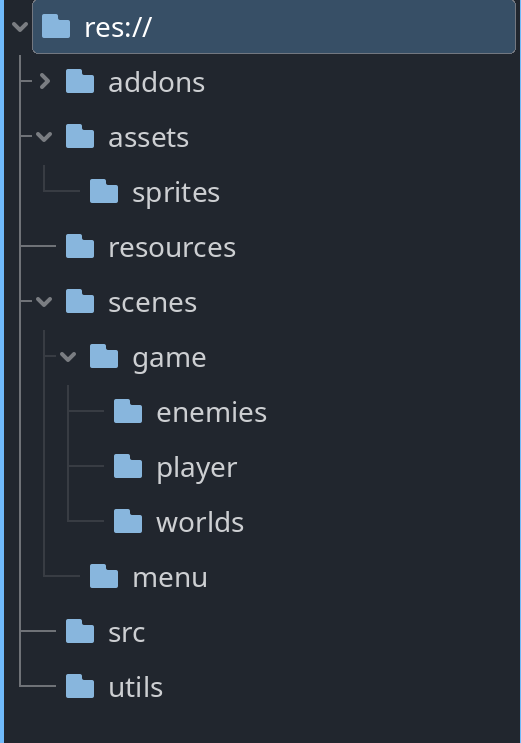
\includegraphics[width = 0.3\textwidth]{images/design/File_System.PNG}
                \caption{Folder Structure}
        \end{figure}
        I chose this folder structure as it will allow me to clearly define where all the different parts of the game are aswell as easily being able to access the closely related parts.\\
        The assets folder will contain all of the external assets, sprites, spritesheets and audio.\\
        The resources folder will contain all of the items (weapons, armour, keys and charms) that I will make to be included in the game.\\
        The scenes folder will contain all the scenes for the menu and the game sorted into their respective folders.\\
        The src folder will contain all of the preloaded scripts for the game.\\
        the utils folder will contain any testing or debugging scripts/scenes to help with the development process.\\
        \subsubsection{Naming Convention}
        For naming I conventions I will adopt the naming conventions already used in godot for ease of integration, readability and consistency with documentation.\\
        The naming conventions are as follows.\\
        \begin{tabular}{|c|c|c|}
                \hline
                Type&Convention&Info\\
                \hline
                File Names&snake\_case&yaml\_parsed.gd\\
                \hline
                Class Names&PascalCase&YAMLParser\\
                \hline
                Node Names&PascalCase&\\
                \hline
                Functions&snake\_case&\\
                \hline
                Variables&snake\_case&\\
                \hline
                Signals&snake\_case& Past tense "door\_opened"\\
                \hline
                Constants&CONSTANT\_CASE&\\
                \hline
        \end{tabular}
        \newpage
        \subsection{Database Design}
        I will be using an SQL Database in order to store the data about my users.\\
        \subsubsection{ERD}
        \begin{figure}[H]
                \centering
                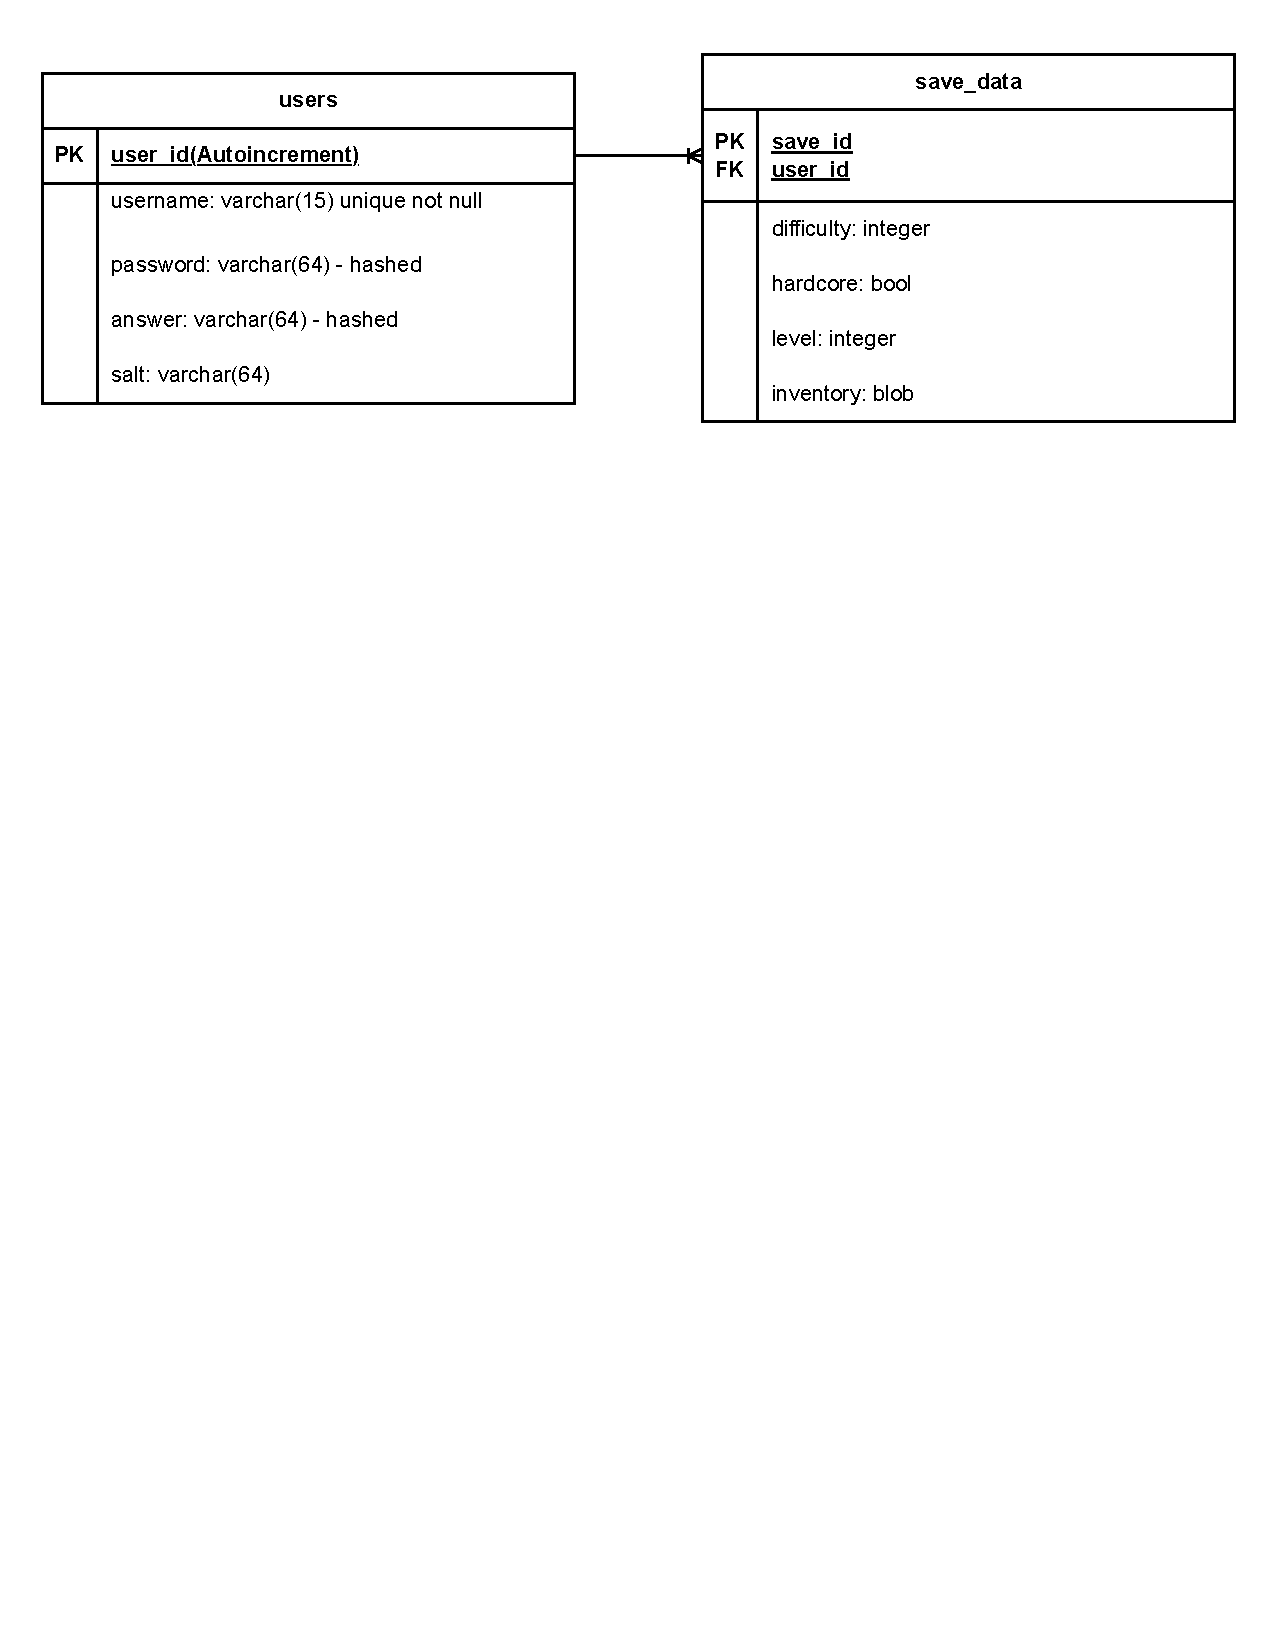
\includegraphics[width=\textwidth, trim = 0 575 0 25, clip]{images/design/Database_Design.pdf}
                \caption{Database Design}
        \end{figure}
        Figure 2 shows the Database Design:\\
        The users table will be the main table containing all the login details.\\
        Each user will be able to have multiple save instances which will be stored in save data.\\
        Upon designing the inventory I have decided that I will split the inventory into the stored items which I will use a seperate table to store with the item\_id (the path to the item resources location in the game files) as a primary composite key with the save \_id aswell as storing the equipped items in the save\_data table. I have also decided to split the composite key in the save\_data table and just have the save\_id as the primary key autoincrementing. This will help keep the inventory more accessible and prevent the need for a BLOB decoder.\\
        \begin{figure}[H]
                \centering
                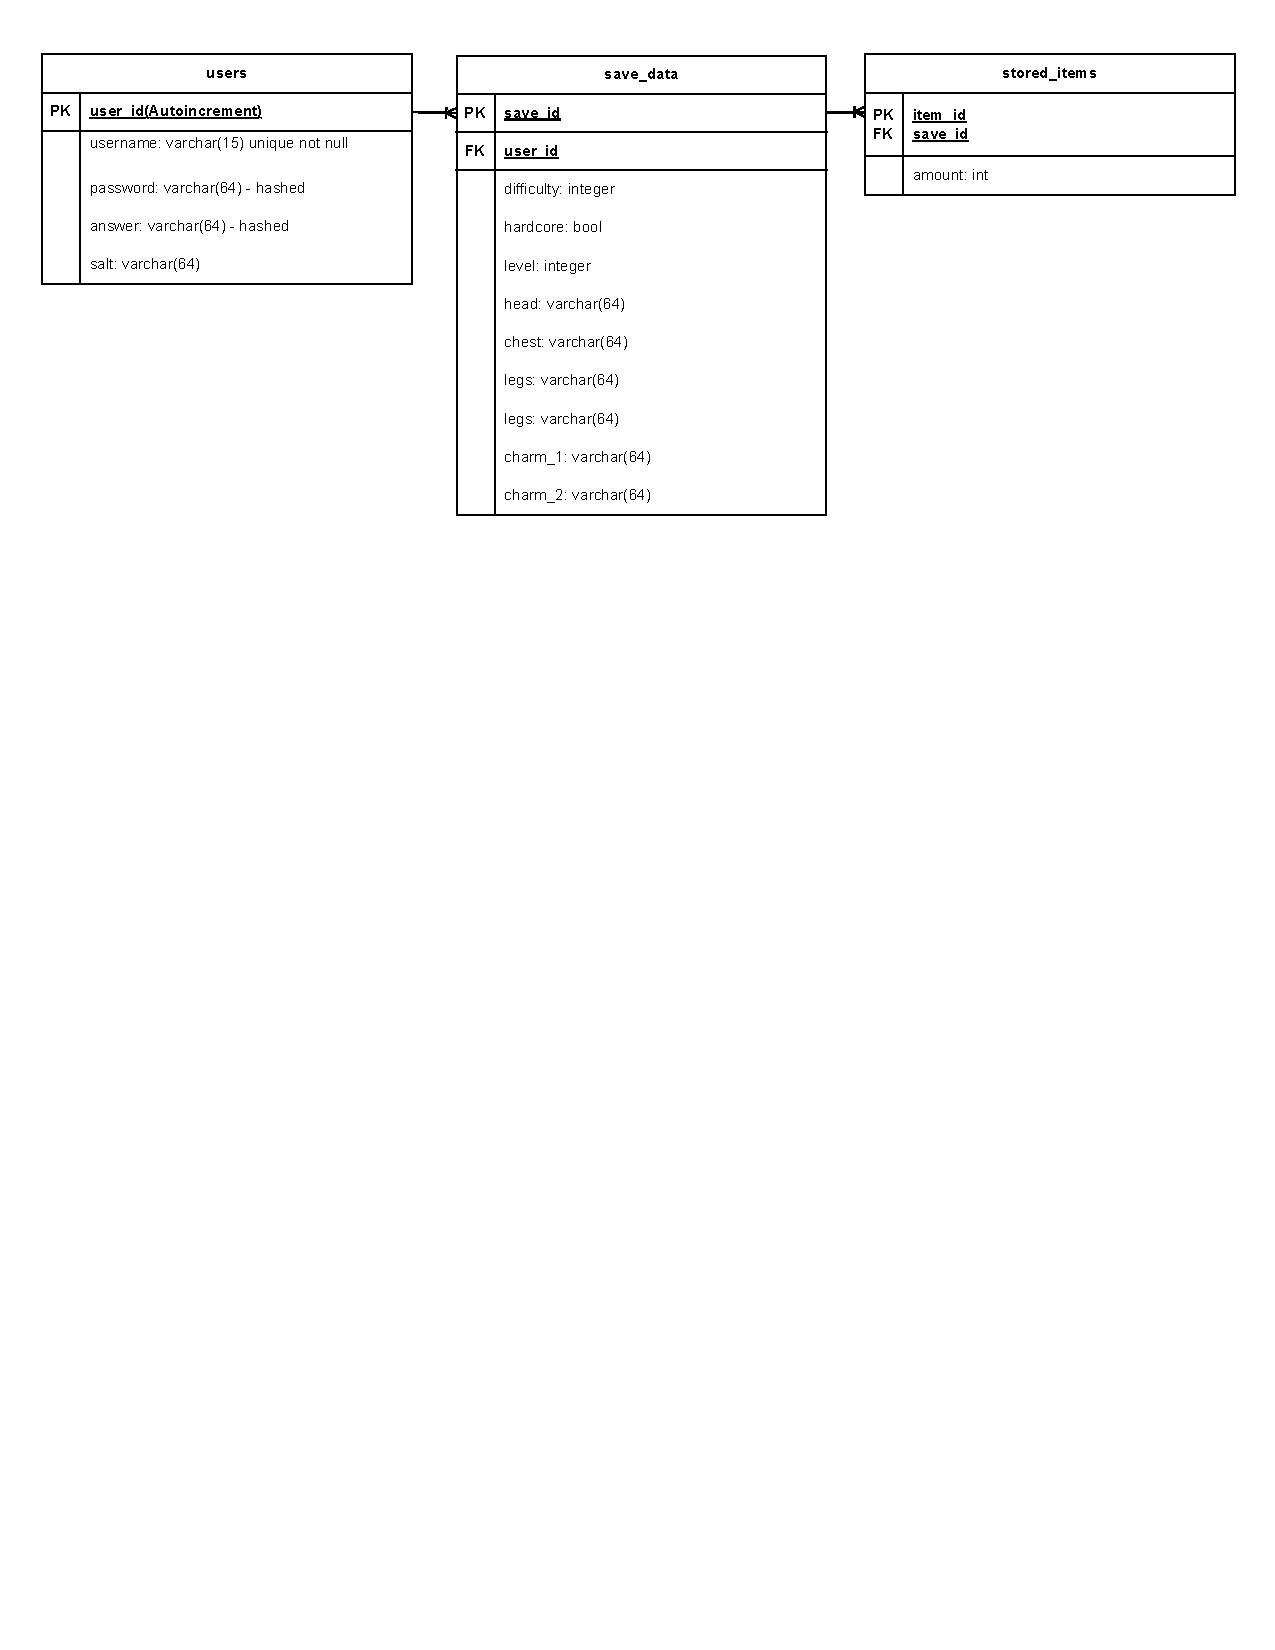
\includegraphics[width=\textwidth, trim = 0 525 0 25, clip]{images/design/Database_Design_Second.pdf}
                \caption{Database Design}
        \end{figure}
        \subsubsection{Database Naming Conventions}
        The naming conventions I will adopt for the database is as follows.\\
        \begin{tabular}{|c|c|c|c|}
                \hline
                Abstract&Convention&Examples&Justification\\
                \hline\
                &&&\\
                Tables&Plural snake\_case&users,save\_data&\mr{7}{4cm}{SQL is case insensitive so with CamelCase it cann't tell the difference between undervalue and underValue}\\
                &&&\\
                \cline{1-3}
                &&&\\
                Fields&Singular snake\_case&inventory\_content, username&\\
                &&&\\
                \cline{1-3}
                &&&\\
                Keys& singular snake\_case\_table\_id&user\_id, save\_data\_id&\\
                &&&\\
                \hline
        \end{tabular}       
        \subsubsection{SQL Queries}
        I have to write Queries for each of the actions I want to do.\\
        \begin{tabular}{|c|c|c|}
                \hline
                Name&Description/Justification&SQL\\
                \hline
                \mr{2}{3.5cm}{create\_table\_users}&\mr{2}{3cm}{Create's a table for users if it does not exist.}&\mr{2}{9.5cm}{\texttt{CREATE TABLE IF NOT EXISTS users (\\\tab user\_id INTEGER PRIMARY KEY AUTOINCREMENT,\\\tab username VARCHAR(15) NOT NULL,\\\tab password VARCHAR(64) UNIQUE NOT NULL,\\\tab salt VARCHAR(64) NOT NULL,\\\tab answer VARCHAR(64) NOT NULL\\);}}\\
                &&\\
                &&\\
                &&\\
                &&\\
                &&\\
                &&\\
                &&\\
                \hline
                \mr{2}{3.5cm}{get\_user\_data}&\mr{2}{3cm}{Returns the user data assuming it exists. If it doesnt it will return null.}&\mr{2}{9.5cm}{\texttt{SELECT * FROM users\\WHERE username = ?;}}\\
                &&\\
                &&\\
                &&\\
                \hline
                \mr{2}{3.5cm}{add\_new\_user}&\mr{1}{3cm}{Inserts a new user into users with username, password, challenge question answer and salt}&\mr{2}{9.5cm}{\texttt{--Assume hashed password and answer\\INSERT INTO\\users(username,password,answer,salt)\\VALUES (?,?,?,?);}}\\
                &&\\
                &&\\
                &&\\
                &&\\
                &&\\
                \hline
                \mr{2}{3.5cm}{reset\_password}&\mr{2}{3cm}{Changes a users password}&\mr{2}{9.5cm}{\texttt{--Assume hashed password and answer\\UPDATE TABLE users\\SET password = ?\\WHERE username = ?}}\\
                &&\\
                &&\\
                &&\\
                \hline
                \mr{3}{3.5cm}{create\_table\_save\_data}&\mr{2}{3cm}{Create's a table for save\_data if it does not exist.}&\mr{2}{9.5cm}{\texttt{CREATE TABLE IF NOT EXISTS save\_data (\\\tab save\_id INTEGER AUTOINCREMENT,\\\tab FOREIGN KEY (user\_id) REFERENCES users(user\_id),\\\tab difficulty INTEGER,\\\tab hardcore INTEGER,\\\tab level INTEGER,\\\tab head VARCHAR(32),\\\tab chest VARCHAR(32),\\\tab legs VARCHAR(32),\\\tab weapon VARCHAR(32),\\\tab charm\_1 VARCHAR(32),\\\tab charm\_2 VARCHAR(32)\\);\\}}\\
                &&\\
                &&\\
                &&\\
                &&\\
                &&\\
                &&\\
                &&\\
                &&\\
                &&\\
                &&\\
                &&\\
                &&\\
                \hline
                \mr{2}{3.5cm}{add\_new\_save\_data}&\mr{2}{3cm}{Adds new save data for a user.}&\mr{2}{9.5cm}{\texttt{INSERT INTO\\save\_data(user\_id,difficulty,hardcore,level)\\VALUES (?,?,?,?);}}\\
                &&\\
                &&\\
                \hline
                \mr{2}{3.5cm}{get\_save\_data}&\mr{2}{3cm}{Get's the save data with a specific user\_id and save\_id}&\mr{2}{9.5cm}{\texttt{SELECT * FROM save\_data\\WHERE user\_id = ?\\AND save\_id = ?;}}\\
                &&\\
                &&\\
                \hline
                \mr{2}{3.5cm}{get\_user\_save\_data}&\mr{2}{3cm}{Get's the save data for all entries with a specific user\_id}&\mr{2}{9.5cm}{\texttt{SELECT level, hardcore FROM save\_data\\WHERE user\_id = ?;}}\\
                &&\\
                &&\\
                \hline
                \mr{2}{3.5cm}{update\_save\_data}&\mr{2}{3cm}{updateSave}&\mr{2}{9.5cm}{\texttt{UPDATE save\_data\\SET\\\tab head = ?,\\\tab chest = ?,\\\tab legs = ?,\\\tab weapon = ?,\\\tab charm\_1 = ?,\\\tab charm\_2 = ?,\\\tab level = ?\\WHERE\\\tab user\_id = ?\\AND save\_id = ?;}}\\
                &&\\
                &&\\
                &&\\
                &&\\
                &&\\
                &&\\
                &&\\
                &&\\
                &&\\
                &&\\
                &&\\
                \hline
        \end{tabular}
        \newpage
        \[\]
        \begin{tabular}{|c|c|c|}
                \hline
                Name&Description/Justification&SQL\\
                \hline
                \mr{2}{4.2cm}{create\_table\_stored\_items}&\mr{2}{2.5cm}{Create's a table for stored\_items if it does not exist.}&\mr{2}{9.3cm}{\texttt{CREATE TABLE IF NOT EXISTS stored\_items (\\item\_id INTEGER NOT NULL,\\save\_id INTEGER NOT NULL,\\PRIMARY KEY(item\_id,save\_id),\\FOREIGN KEY(save\_id) REFERENCES save\_data(save\_id)\\);}}\\
                &&\\
                &&\\
                &&\\
                &&\\
                &&\\
                \hline
                \mr{2}{4.2cm}{update\_stored\_item\_amount}&\mr{2}{2.5cm}{Update's a specific person's stored items to increase the amount of something stored (assumes it is stored)}&\mr{2}{9.3cm}{\texttt{UPDATE stored\_items\\SET amount = amount + ?\\WHERE item\_id = ?\\AND save\_id = ?;\\}}\\
                &&\\
                &&\\
                &&\\
                &&\\
                &&\\
                &&\\
                &&\\
                \hline
                \mr{2}{4.2cm}{get\_stored\_item\_amount}&\mr{2}{2.5cm}{Get's the amount of an item being stored}&\mr{2}{9.3cm}{\texttt{SELECT amount FROM stored\_items\\WHERE save\_id = ?\\AND item\_id = ?;}}\\
                &&\\
                &&\\
                &&\\
                &&\\
                \hline
                \mr{2}{4.2cm}{add\_stored\_item}&\mr{2}{2.5cm}{Adds an item to the stored\_items}&\mr{2}{9.3cm}{\texttt{INSERT INTO\\stored\_items(save\_id,item\_id,amount)\\VALUES (?,?,?);}}\\
                &&\\
                &&\\
                \hline
                \mr{2}{4.2cm}{count\_stored\_items}&\mr{2}{2.5cm}{Count's the number of items stored for a save\_id}&\mr{2}{9.3cm}{\texttt{SELECT COUNT(*)\\FROM stored\_items\\WHERE save\_id = ?;}}\\
                &&\\
                &&\\
                &&\\
                \hline
                \mr{2}{4.2cm}{remove\_stored\_item}&\mr{2}{2.5cm}{Removes an item from stored\_items}&\mr{2}{9.3cm}{\texttt{DELETE * FROM stored\_items\\WHERE save\_id = ?\\AND item\_id = ?;}}\\
                &&\\
                &&\\
                \hline
                \mr{2}{4.2cm}{get\_slot\_value}&\mr{2}{2.5cm}{Gets the file path of the item equipped in the slot}&\mr{2}{9.3cm}{\texttt{SELECT ? FROM save\_data\\WHERE save\_id = ?;}}\\
                &&\\
                &&\\
                &&\\
                \hline
                \mr{2}{4.2cm}{set\_slot\_value}&\mr{2}{2.5cm}{Sets the value of the slot to the file path}&\mr{2}{9.3cm}{\texttt{UPDATE save\_data\\ SET ? = ?\\WHERE save\_id = ?;}}\\
                &&\\
                &&\\
                \hline
                \mr{2}{4.2cm}{}&\mr{2}{2.5cm}{}&\mr{2}{9.3cm}{\texttt{}}\\
                &&\\
                \hline
        \end{tabular}
        I will use godot's $query\_with\_bindings()$ function in order to substitute in the bindings for the ?s in the queries. This is useful as it automatically performs input sanitisation so that the system isn't vulnerable to SQL injection.\\
        \subsubsection{Algorithms}
        \textbf{login():}\\
        The login function will be used to find if the user exists and then check the hashed password if it does. This will help fulfill criteria 6.6.\\
        \begin{python}
def login(username,password):
   query_result = get_user_data(username) #Getting user data
   if len(query_result) == 0: #If user doesnt exist
      return "InvalidUsernameError" 
   if hash(password) == query_result["password"]: #Checking password hash against stored hash
      return True
   return "IncorrectPasswordError" #If password doesnt match
        \end{python}
        \textbf{add\_user():}\\
        The add\_user function will be used to generate salt for the user check if the username is unique and add the user. This will help fulfill criteria 6.3\\
        \begin{python}
def add_user(username, password, answer):
   salt = gen_salt() #Generating new salt
   hashed_password = hash(password,salt)
   hashed_answer = hash(answer,salt)
   if not add_new_user(username, hashed_password, hashed_answer, salt): #Tries to add user with hashed password and answer
      return "InvalidUsernameError" #If user cannot be added then the username must be invalid
   return True
        \end{python}
        \textbf{reset\_password():}\\
        The reset\_password function will be used to check if the username is valid, fetch the user data and then check if the hashed answer is the same as the stored answer before updating the stored password. This will help fulfill criteria 6.7.\\
        \begin{python}
def reset_password(username, answer, password):
   query_result = get_user_data(username) #Getting user data
   if len(query_result) == 0: #If user doesnt exist
      return "InvalidUsernameError"
   if hash(answer) == query_result["answer"]: #Checking the answer hash against the stored hash
      reset_password(password,username)
      return True
   return "IncorrectAnswerError" #If answer doesnt match
        \end{python}
        \subsubsection{Testing Plan}
        \begin{tabular}{|c|c|c|c|}
                \hline
                Test \#&Function&Parameters&Expected Outcome\\
                \hline
                6.3.1&add\_user()&"Hyrule", "Password", "Answer"&\mr{2}{6cm}{True}\\
                &&&\\
                \hline
                6.3.2&add\_user()&"Hyrule", "Password", "Answer"&\mr{2}{6cm}{"InvalidUsernameError" as a user already exists with that username}\\
                &&&\\
                \hline
                6.6.1&login()&"Hyru1e", "Password"&\mr{2}{6cm}{"InvalidUsernameError"}\\
                &&&\\
                \hline
                6.6.2&login()&"Hyrule", "Password"&\mr{2}{6cm}{True}\\
                &&&\\
                \hline
                6.7.1&reset\_password()&"Hyru1e", "Answer", "password&\mr{2}{6cm}{"InvalidUsernameError"}\\
                &&&\\
                \hline
                6.7.2&reset\_password()&"Hyrule", "answer", "password"&\mr{2}{6cm}{"IncorrectAnswerError"}\\
                &&&\\
                \hline
                6.7.3&reset\_password()&"Hyrule", "Answer", "password"&\mr{2}{6cm}{True}\\
                &&&\\
                \hline
                6.6.3&login()&"Hyrule", "Password"&\mr{2}{6cm}{"IncorrectPasswordError"}\\
                &&&\\
                \hline
                &&&\mr{2}{6cm}{}\\
                &&&\\
                \hline
        \end{tabular}
        These tests will be used to evaluate to what extent I have met the criteria and allow me to identify and fix any issues in my code.\\
        \subsection{Login System}
        \subsubsection{Activity Diagram}
        \begin{figure}[H]
                \centering
                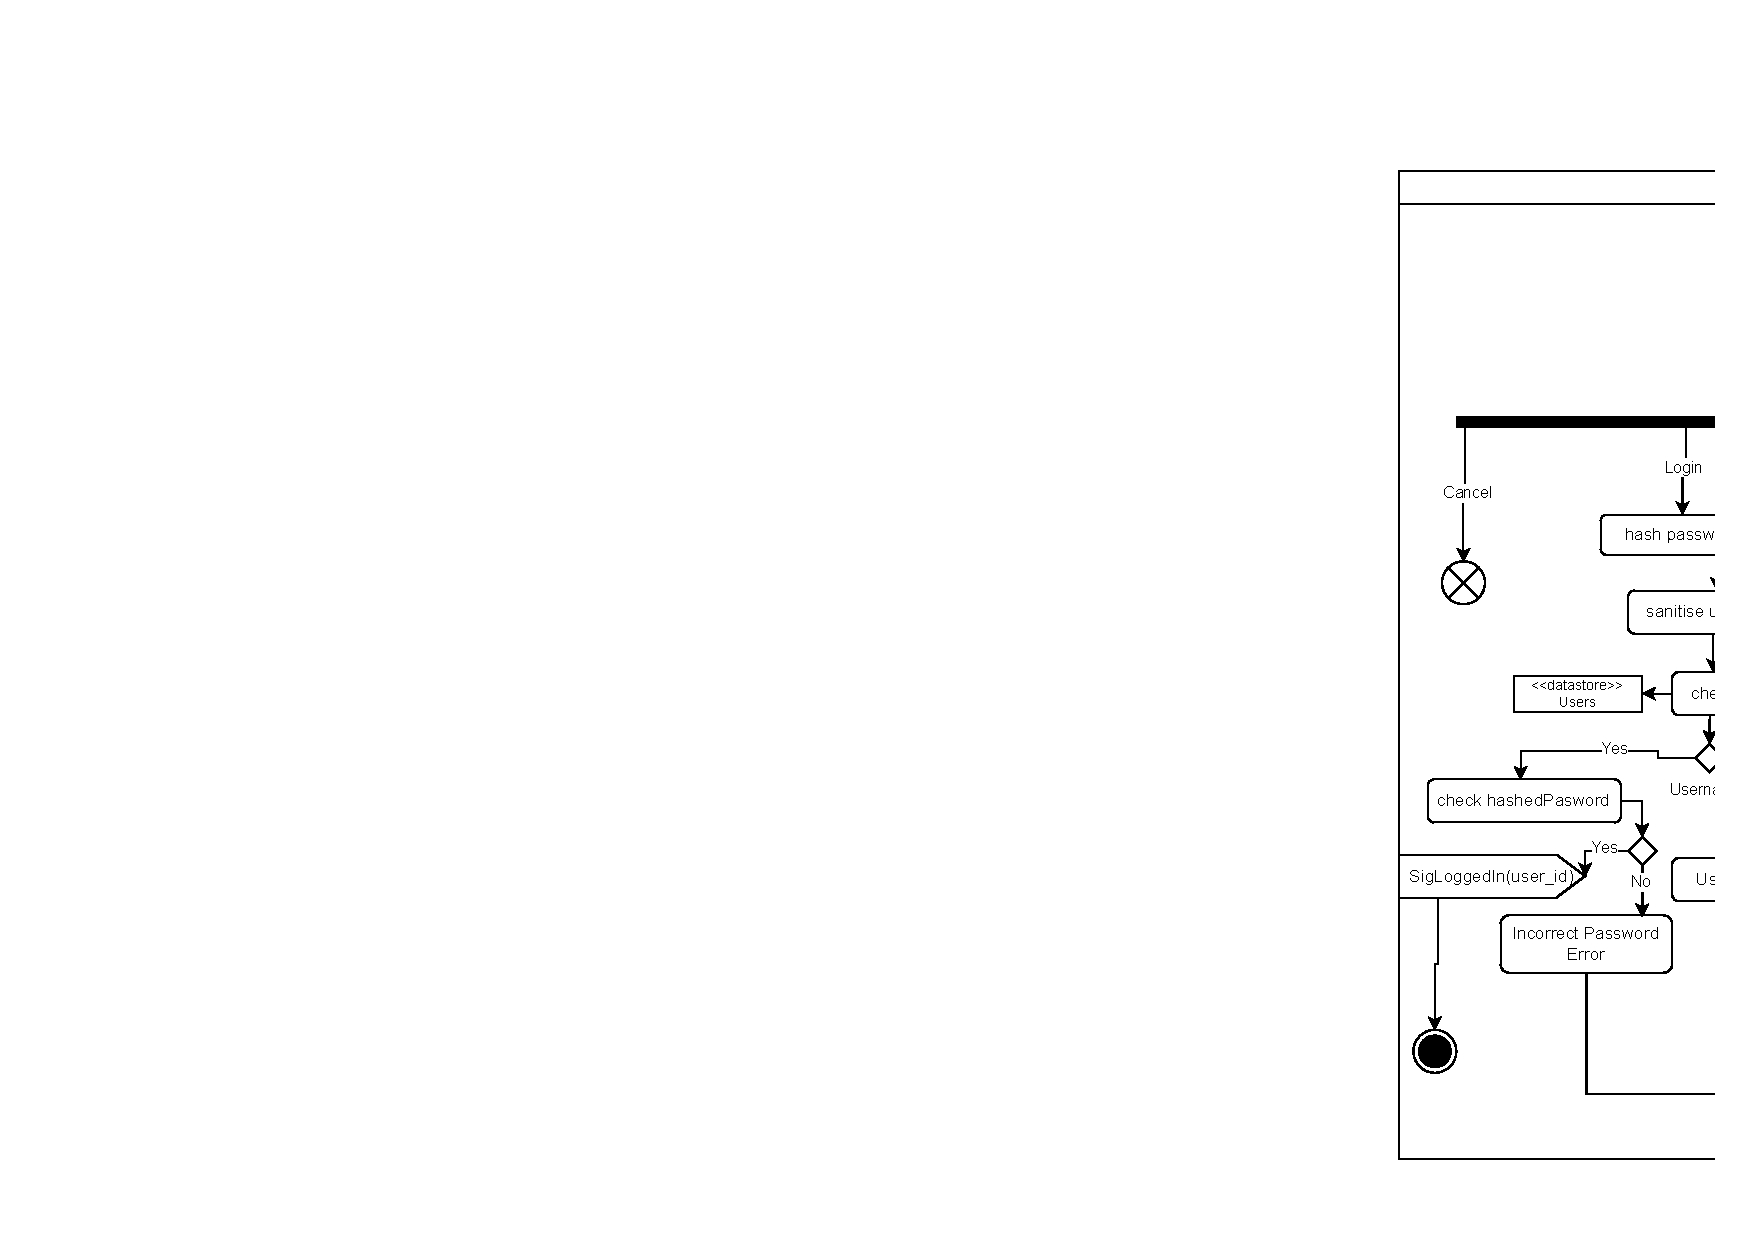
\includegraphics[width=\textwidth, trim = 0 50 0 0, clip]{images/design/Login_System.pdf}
                \caption{Activity Diagram for login forms}
                
        \end{figure}
        The login form will allow users to create accounts aswell as login with an existing account and reset a password.\\
        Upon successful login the user will be redirected to the GAME system. This login form along with the database functions provides all the necessary UI and algorithmic elements to fulfill criteria 6.\\
        \subsubsection{Algorithms}

        \textbf{hash():}\\
        This function alternates between two different hashing functions a consistent number of times while making sure the final hash is a consistent length. It also adds in a unique salt for every user which is necessary to prevent rainbow table lookups and keep the passwords secure even if it is generic. This and the salt function fulfills criteria 6.1.\\
        \begin{python}
def hash(password: str, salt: str):
   hashedPassword = password
   #Repeating a consistent but unpredicatble amount of times
   #On even rounds the password is sandwidged on odd rounds the salt is sandwidged
   #Alternating the use of sha256 and md5 but making sure to end on sha256 so the hash is a predictable length.
   for x in range(1,6*len(password)+1):
      if x\%2 == 0:
         hashedPassword = sha256(md5(salt[x:]+hashedPassword+salt[:x]))
      else:
         hashedPassword = md5(sha256(hashedPassword[:x]+salt+hashedPassword[x:]))
        return hashedPassword
        \end{python}
        \textbf{genSalt():}\\
        The genSalt function uses random processes to generate a salt string to be used in the hashing of the password and challenge question. This needs to be random for every user to prevent the potential to create a table of common password hashes to loop up user's passwords in.\\
        \begin{python}
def gen_salt():
   salt = "string"
   x = randint(5,10)
   for i in range(2**x):
      salt = hash(salt,sha256(str(i)))
   return salt
        \end{python}
        \subsubsection{Testing Plan}
        \begin{tabular}{|c|c|c|c|}
                \hline
                Test \#&Function&Parameters&Expected Outcome\\
                \hline
                6.1.1&gen\_salt()&&\mr{2}{6cm}{random 256 bit hex string}\\
                &&&\\
                \hline
                6.1.2&hash()&"password", "salt"&\mr{2}{6cm}{random 256 bit hex string}\\
                &&&\\
                \hline
                6.1.3&hash()&"password", "salt"&\mr{2}{6cm}{the same random 256 bit hex string}\\
                &&&\\
                \hline
                6.1.2&hash()&"Password", "salt"&\mr{2}{6cm}{random 256 bit hex string different from before}\\
                &&&\\
                \hline
        \end{tabular}
        \subsubsection{Mockup Forms}
        \begin{multicols}{3}
                \begin{figure}[H]
                        \centering
                        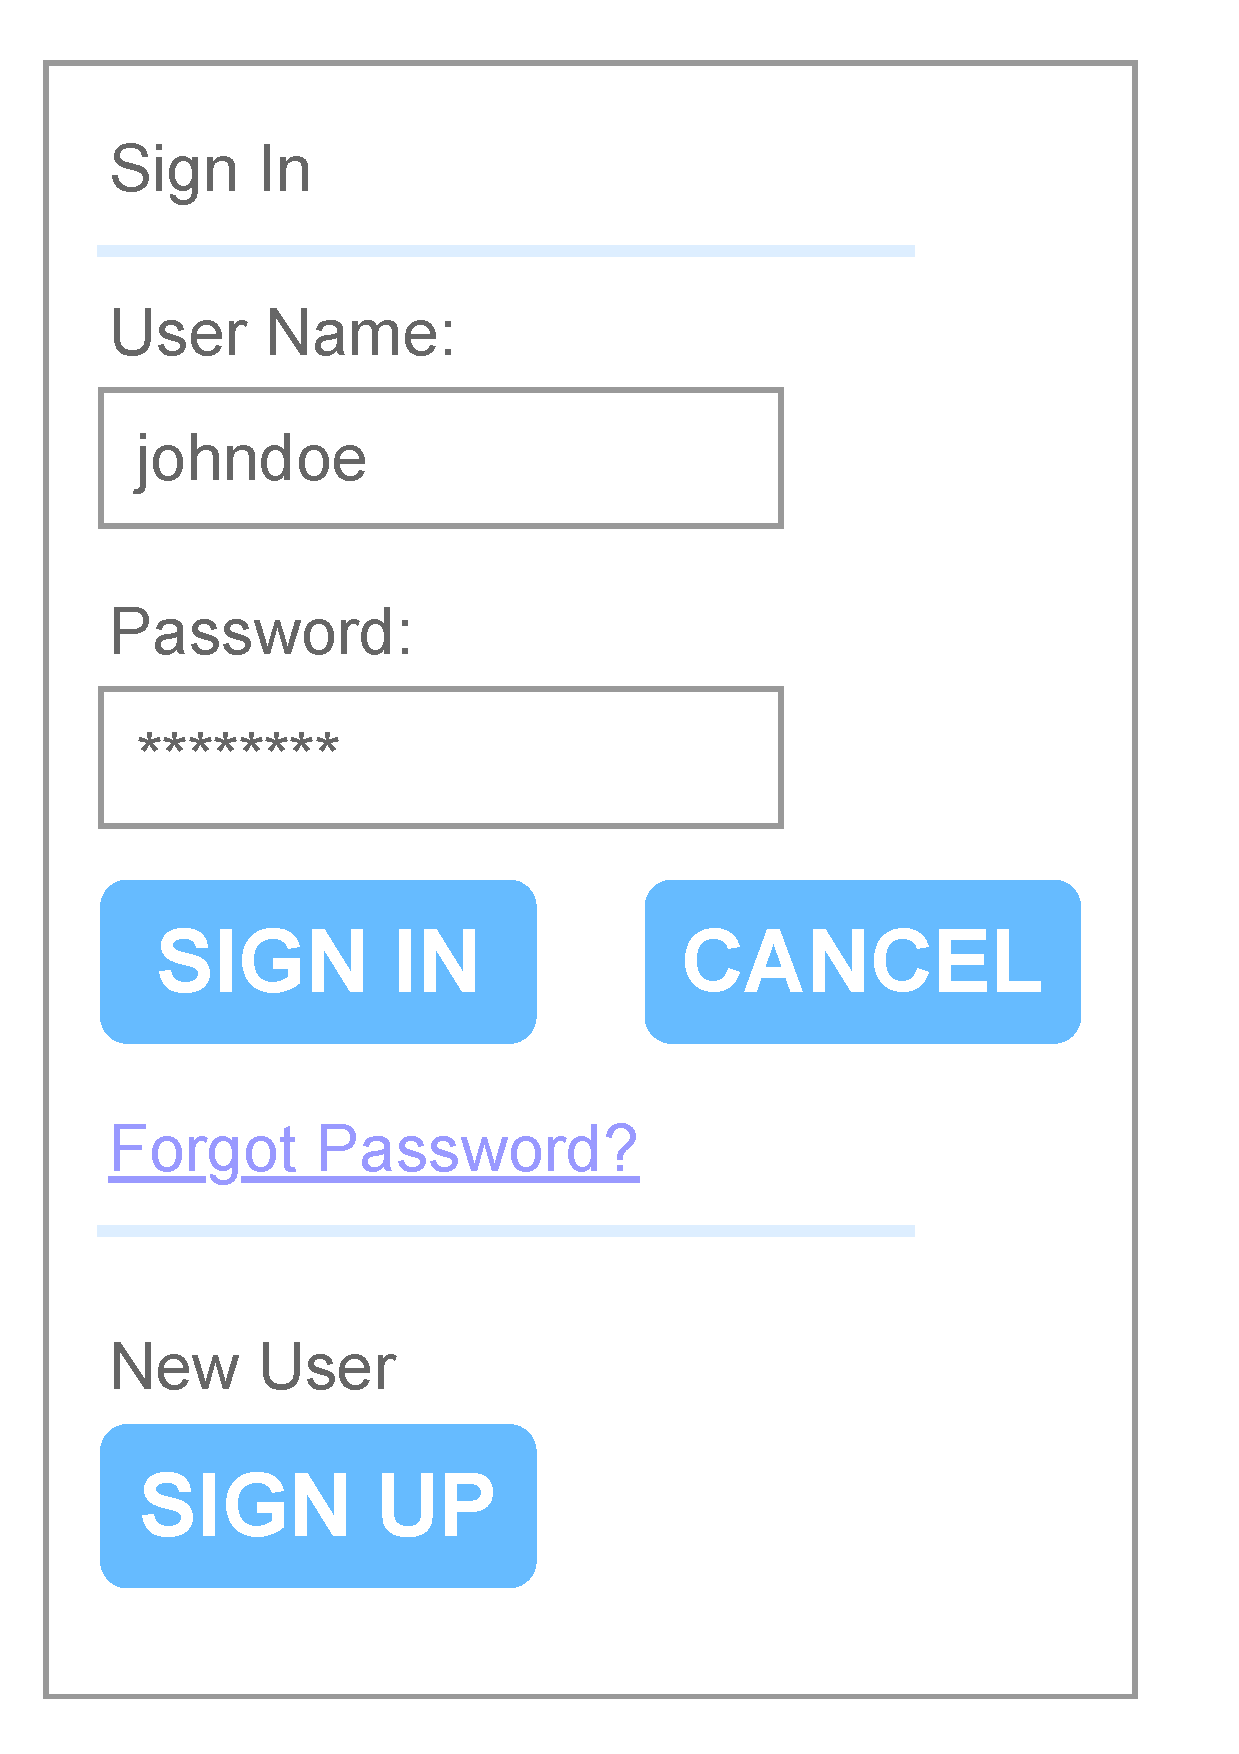
\includegraphics[width = 0.9\columnwidth]{images/design/Login_Form.pdf}
                        \caption{Login Form}
                \end{figure}
                \begin{figure}[H]
                        \centering
                        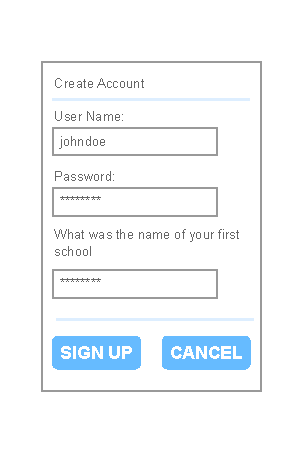
\includegraphics[width = 0.9\columnwidth]{images/design/Sign_Up_Form.pdf}
                        \caption{New Account Form}
                \end{figure}
                \begin{figure}[H]
                        \centering
                        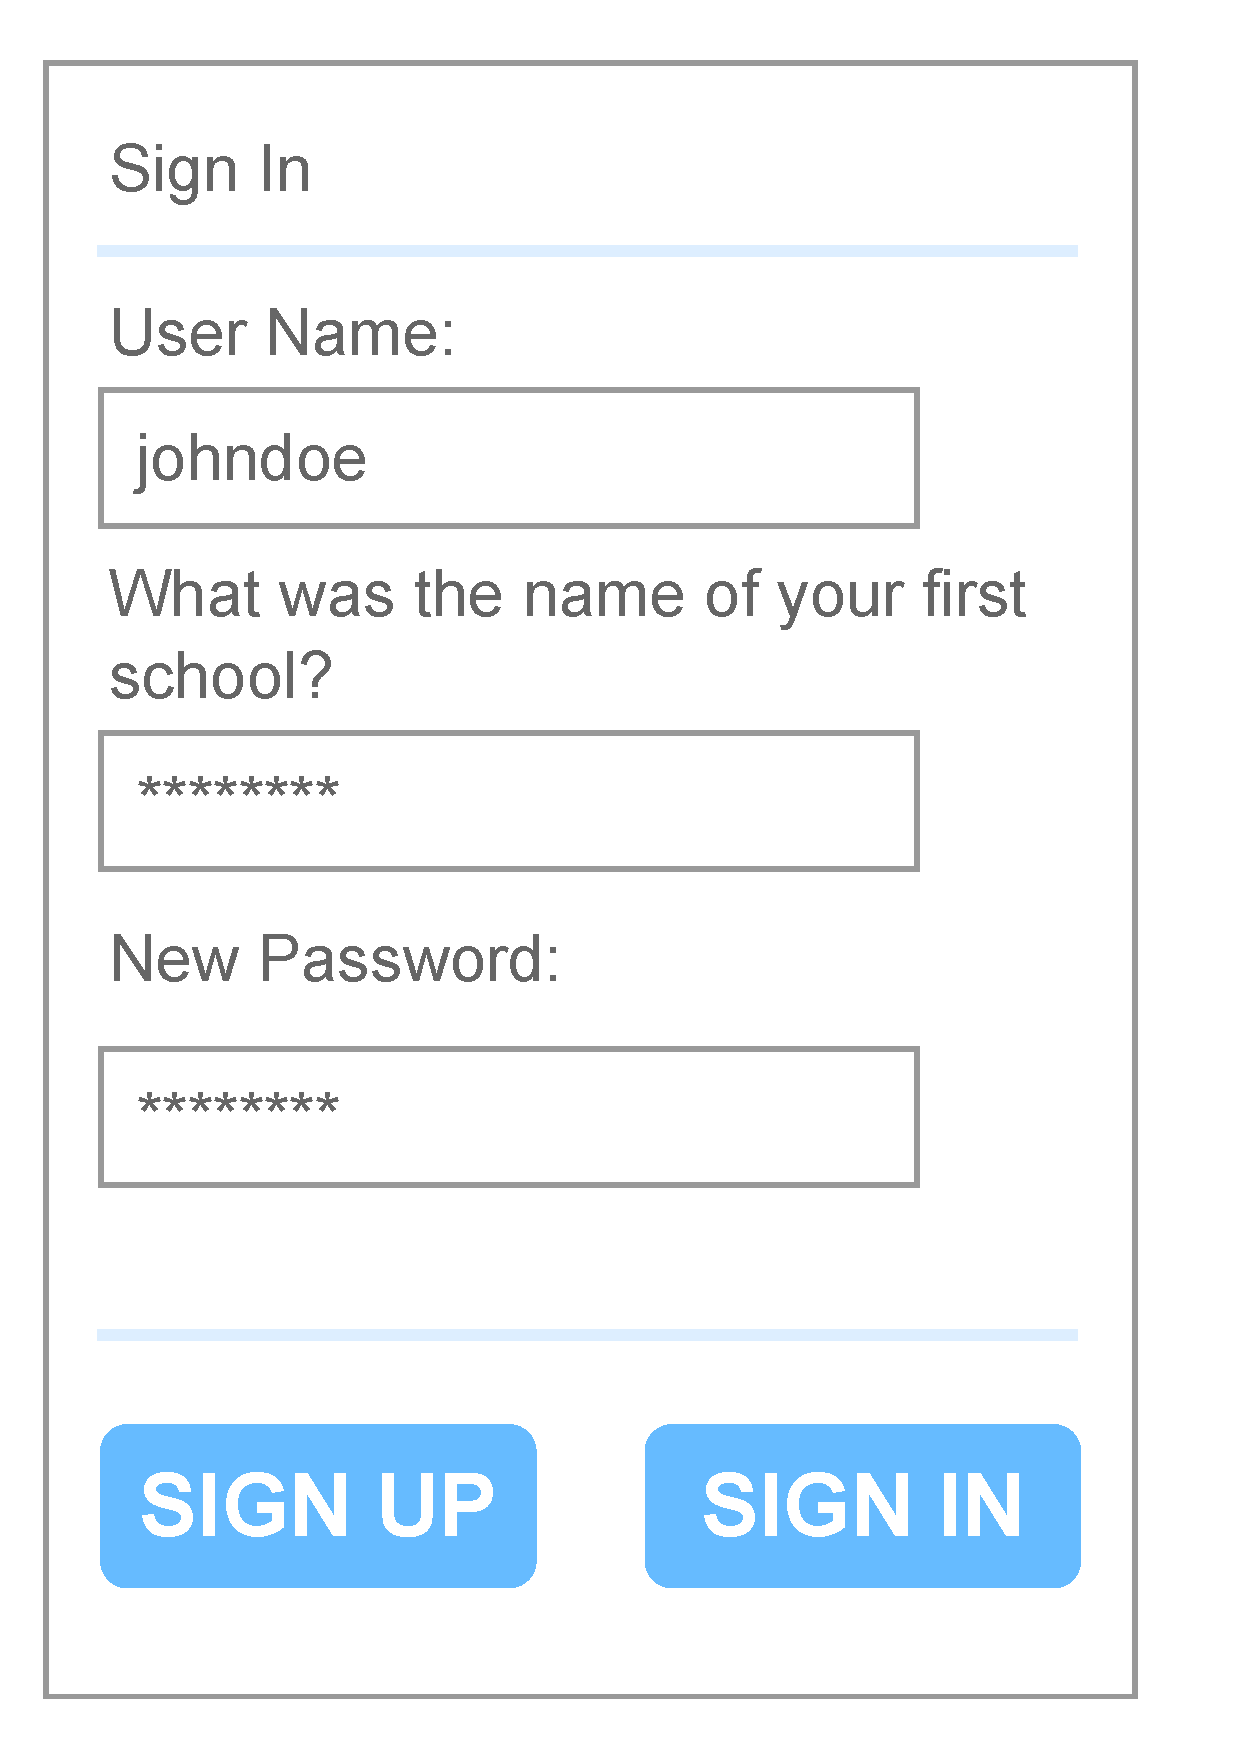
\includegraphics[width = 0.9\columnwidth]{images/design/Reset_Password.pdf}
                        \caption{Reset Password Form}
                \end{figure}
        \end{multicols}\[\]
        These forms would be used in order to create an account, reset your password and login, Helping fulfill criteria 6.3, 6.6, 6.7 and 6.8.\\
        The Password and Challenge question entries would be hidden/starred for privacy.\\
        \newpage
        \subsection{Save Select System}
        I will implement the save select system as an additional menu for the login system in order to improve replayability to help  using a ScrollContainer with a VBoxContainer inside to create a list of scrollable items. I will get the list of saves for a given user\_id and then display them and when the button for that save is pressed the current\_save\_id will be set.\\
        In order to add new save's I will add a button for hardcore and a slider for difficulty as well as an add save button which will add the save and update the list.\\
        \subsubsection{Algorithms}
        \textbf{\_ready():}
        \begin{python}
def _ready():
   save_data_list = get_user_save_data(current_user_id)
   for save_data in save_data_list:
      button = Button.new
      button.text = f"Level: {save_data['level']} \t Difficulty: {save_data['difficulty']}\n Hardcore: {save_data['hardcore']}"
      button.connect("pressed", self, "_on_save_selected", [save_data])
      add_child(button)
        \end{python}
        \textbf{\_on\_save\_selected():}
        \begin{python}
def _on_save_selected(save_data):
   current_save_id = save_data["save_id"]
   get_tree().change_scene_to_file(world)
        \end{python}
        \subsection{Item Design}
        I will implement the different item types using Godot's resource system. This will allow me to define properties that all items of the same type will share and I can use inheritance to allow classes to derive from a parent class.\\
        The resource system is useful as it is reusable throughout scenes and scripts and it can easily be saved and loaded from disk.\\
        The types of items I will aim to implement will be different weapon types, charms/trinkets/amulets, armour and keys.\\
        \subsubsection{Class Diagram}
        \begin{figure}[H]
                \centering
                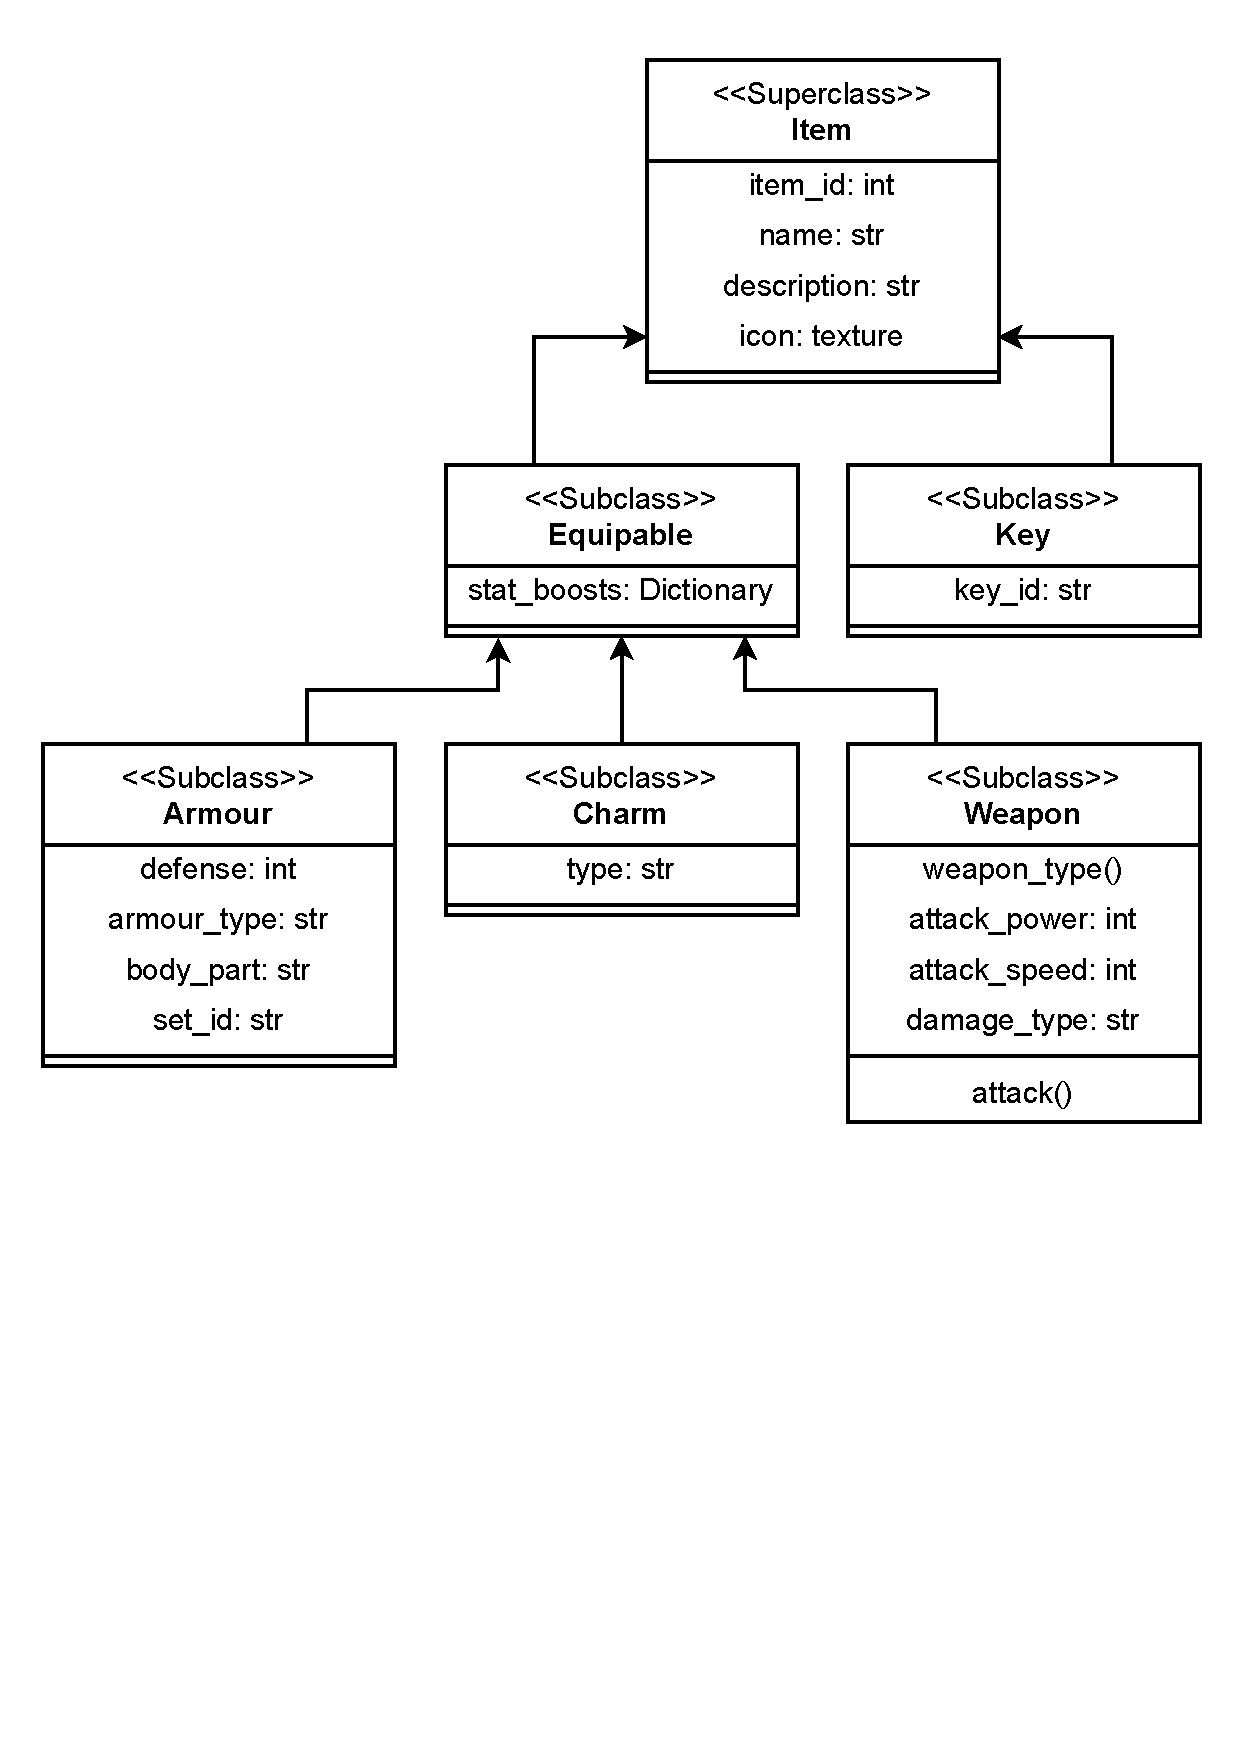
\includegraphics[width = 0.9\columnwidth, clip, trim = 0 270 0 25]{images/design/Item_Class_Diagram.pdf}
                \caption{Player Class Diagram}
        \end{figure}
        \subsubsection{Algorithms}
        \textbf{attack():}\\
        I will have a number of different weapon types that will have different attacks.\\
        I will implement the attack cooldown through the use of a CooldownTimer(timer node) attached to the player.\\
        Melee:\\
        I will implement the melee attack by creating a variable size hitbox(area2D) scene that can be instantiated as a child of the player in order to detect enemies that would be attacked in the range specified in the resource.\\
        \begin{python}
def attack(owner: node, direction):
   #Load the hitbox scene
   hitbox_scene = load(hitbox_scene_path)
   hitbox_instance = hitbox_scene.instantiate()
   hitbox_instance.range = range
   hitbox_instance.damage = damage
   hitbox_instance.rotation = direction.angle()

   #Add child
   owner.add_child(hitbox_instance)

   #Hitbox lasts for a tenth of a second
   sleep(0.1)
   
   hitbox_instance.queue_free()

        \end{python}
        Ranged:\\
        My Bows and ranged magic weapons will shoot out projectiles.
        \begin{python}
def attack():
   #Load the projectile scene
   projectile_scene = load(projectile_scene_path)
   projectile_instance = projectile_scene.instantiate()
   projectile_instance.damage = damage

   #Add Child
   owner.add_child(projectile_instance)
        \end{python}
        \textbf{display\_string():}
        Upon designing the Inventory UI I have decided to add a function to output a string describing the item, this would make use of polymorphism to behave differently for each item and display the key stats like the name, stat\_boosts and such.\\
        \subsection{Inventory Design}
        My inventory design will cover two main parts the equipped items and the item storage. I will have a maximum inventory size script variable so that we can still display all the items in the inventory and a max stack size for stackable items.\\
        \subsubsection{Stored Items}
        I will implement the stored items through a dictionary that stores the item resource and the quantity of it. I will implement add and remove item functions. I will also add a max inventory size.\\
        \subsubsection{Equipped Items}
        I will implement the equipped items through a dictionary where the keys are the slots and the values are what is equipped in that slot. I will also add a equip function to equip an item and an unequip function to unequip the item in a slot.\\
        \subsubsection{Clarification}
        Upon further thought I have decided it is best to use SQL tables instead of dictionaries and use SQL queries to manage the inventory.\\
        \subsubsection{Algorithms}
        \textbf{add\_item():}\\
        \begin{python}
def add_item(item_id: file_path, amount):
   if get_stored_item_amount(save_id, item_id) and item.stackable: #Checks if you can stack the item
      update_stored_item_amount(amount, item_id, save_id)
   elif count_stored_items(save_id) >= max_inventory_size: #Full Inventory
      return "FullInventoryError"
   else:
      add_stored_item(save_id, item_id, amount)
   return True
        \end{python}
        \textbf{remove\_item():}\\
        \begin{python}
def remove_item(item_id: Resource, amount: int = 1):
   if get_stored_item_amount(save_id, item_id): #If the item is in the database
      if get_stored_item_amount(save_id, item_id) < amount: #Not enough items
         return "ItemQuantityError"
      if get_stored_item_amount(save_id, item_id) == amount: #Exactly enough items
         remove_stored_item(save_id, item_id)
      else:
         update_stored_item_amount(-amount, item_id, save_id) #Removes the ammount of that item
      return True #Indicates that it was successful
   return "ItemQuantityError" #Indicates that there is an item quantity error
        
        \end{python}
        \textbf{unequip\_item():}\\
        \begin{python}
def unequip_item(slot: str):
   #Checks if there is an item to unequip
   if get_slot_value(slot, save_id) != null:
      item = get_slot_value(slot, save_id)
      if (add_item(item, 1) == "FullInventoryError"): #Adds the item back to the stored_items and checks if the inventory is full
         return "FullInventoryError"     
      set_slot_value(slot, null, save_id) #Sets the slot back to null
      return True
   return True #If not item in slot it is unequipped
        \end{python}
        \textbf{equip\_item():}\\
        \begin{python}
def equip_item(item: Resource):
        #Checks if the item is Equipable
        if not(item.is_class(Equipable)):
                return False
        #Gets the slot to equip it into
        if item.is_class(Armour):
                slot = item.body_part
        elif item.is_class(Weapon):
                slot = "weapon"
        else:
                equipped = false
                #Tries both charm slots
                for slot in ["charm1","charm2"]:
                        if get_slot_value(slot, save_id) == null and not(equipped):
                                set_slot_value(slot, item, save_id) #Equips item
                                remove_item(item) #Removes from stored_items
                                equipped = True
                if not(equipped):
                        unequip_item(slot)
                        set_slot_value(slot, item, save_id) #Equips item
                        remove_item(item) #Removes from stored_items
                return True
        unequip_item(slot)
        set_slot_value(slot, item, save_id) #Equips item
        remove_item(item) #Removes from stored_items
        return True     
        \end{python}
        \subsubsection{Testing Plan}
        \begin{tabular}{|c|c|c|c|}
                \hline
                Test \#&Function&Parameters&Expected Outcome\\
                \hline
                12.5.1&add\_item()&"test\_item.tres", 2&\mr{2}{6cm}{Adds test item to the stored\_items table.}\\
                &&&\\
                \hline
                12.5.2&add\_item()&"test\_item.tres", 3&\mr{2}{6cm}{As the item already exists it should add 3 to the amount.}\\
                &&&\\
                \hline
                12.5.3&add\_item()&"test\_weapon.tres", 1&\mr{2}{6cm}{As in the testing environment the max inventory size will be 1 and this should return "FullInventoryError"}\\
                &&&\\
                &&&\\
                \hline
                12.5.4&remove\_item()&"test\_item.tres", 2&\mr{2}{6cm}{As more than the amount of the item is in the inventory it should subtract 2.}\\
                &&&\\
                \hline
                12.5.5&remove\_item()&"test\_item.tres", 10&\mr{2}{6cm}{"ItemQuantityError" as there isnt enough of the item in the database}\\
                &&&\\
                \hline
                12.5.6&remove\_item()&"test\_item.tres", 3&\mr{2}{6cm}{As exactly the amount is in the database the item entry should get removed.}\\
                &&&\\
                &&&\\
                \hline
                12.5.7&remove\_item()&"test\_item.tres", 2&\mr{2}{6cm}{"ItemQuantityError" as there isnt any of the item in the database}\\
                &&&\\
                \hline
                12.4.1&unequip\_item()&"head"&\mr{2}{6cm}{True and the head slot should remain as NULL}\\
                &&&\\
                \hline
                12.4.2&equip\_item()&"test\_helmet.tres"&\mr{2}{6cm}{True and the head slot should become "test\_helmet.tres"}\\
                &&&\\
                \hline
                12.4.3&equip\_item()&"test\_helmet\_2.tres"&\mr{2}{6cm}{True and the head slot should become "test\_helmet.tres"}\\
                &&&\\
                \hline
                12.4.4&unequip\_item()&"head"&\mr{2}{6cm}{"FullInventoryError"}\\
                &&&\\
                \hline
                12.4.5&unequip\_item()&"head"&\mr{2}{6cm}{True as I will empty the inventory and the head should be NULL and the inventory should contain the helmet.}\\
                &&&\\
                &&&\\
                \hline
                &&&\mr{2}{6cm}{}\\
                &&&\\
                \hline
        \end{tabular}
        \newpage
        \subsection{Player Character}
        This is my design for the physical player character and sprite.\\
        \subsubsection{Composition}
        \begin{figure}[H]
                \centering
                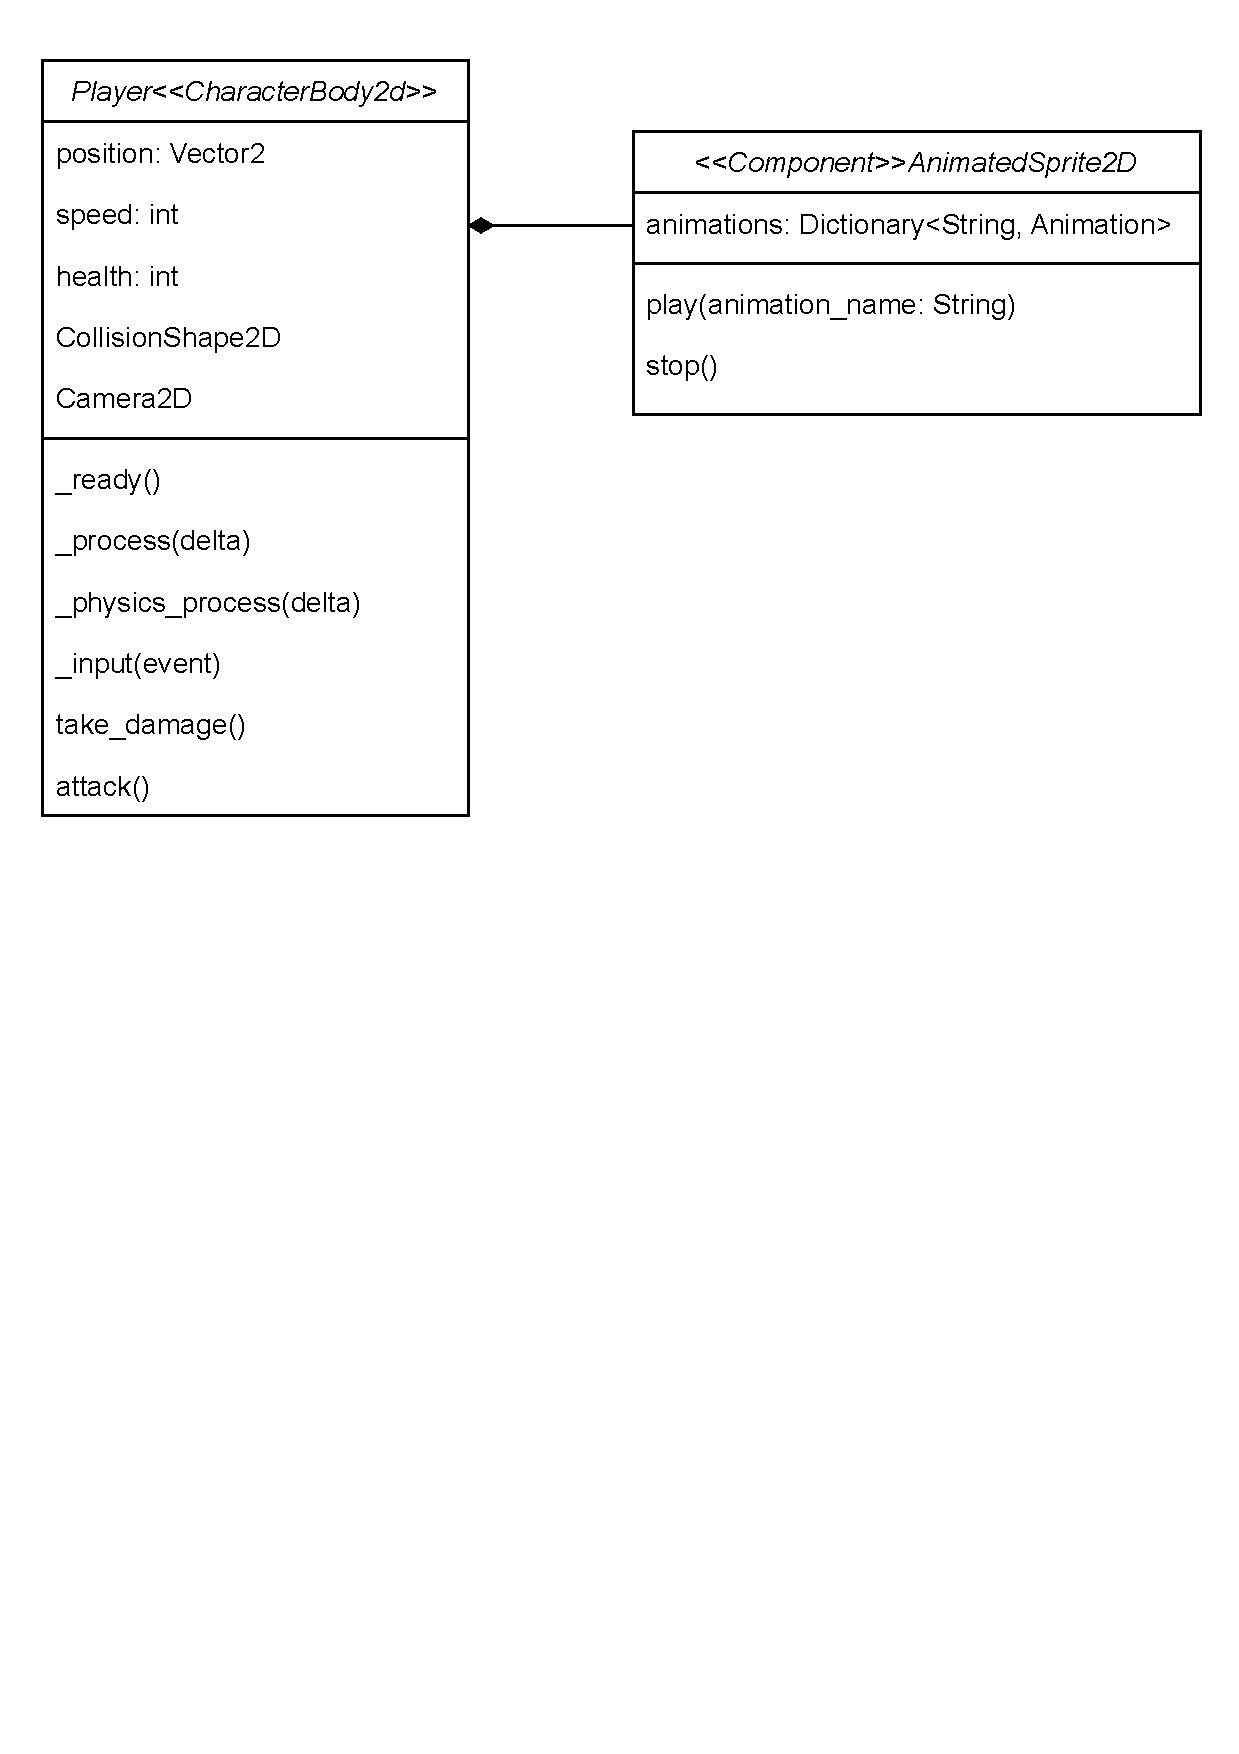
\includegraphics[width = 0.9\columnwidth, clip, trim = 0 450 0 0]{images/design/Player_Class_Diagram.pdf}
                \caption{Player Class Diagram}
        \end{figure}
        The root node of the player which will contain all the child nodes will be Godot's CharacterBody2D as this will allow for a user controlled physics body. It will then have child nodes of CollisionShape2D(for collision detection), AnimatedSprite2D(for an animated character sprite) and Camera2D(for the player's view window to be centered on).\\
        I have chosen to store the speed and health variables within the player class as they will reset/ be recalculated based of the equipment equipped.\\
        \subsubsection{Animations}
        I have an animation set for the player that includes 8 Directional top down animations for all player actions and so how I will decide which directional animation will be based of the last direction the player walked.\\
        I will use a get\_animation function in order to get the directional animation to play.\\
        \subsubsection{Help Screen}
        I have decided to add a simple Help Screen in order to allow the user to check the controls when they want a reminder. I will implement this by creating a seperate scene with a label and then when the help button is pressed I will pause the tree and instance the scene before waiting for the help button to be pressed again to unpause the scene tree and queue\_free the label.\\
        \subsubsection{Algorithms}
        \textbf{\_ready():}\\
        The \_ready() function gets called whenever the player is instantiated in a scene and so it will be used to setup variables and the environment based on existing stuff.\\
        \begin{python}
def _ready():
        #Inventory calculates the speed based on any modifiers equipped.
        speed = Inventory.calc_speed() 
        #Global Script calculates the health based on the player level and any modifiers equipped.
        health = Global.calc_health()
        \end{python}
        \textbf{\_physics\_process(delta):}\\
        The \_physics\_process(delta) function gets called every frame where delta is the time since the last fram and is usually used to deal with movement and physics processes.\\
        \begin{python}
def _physics_process(delta):
   direction = Input.get_vector("left", "right", "up", "down")
   velocity = direction * speed
   if direction:
      last_direction = direction
      anim.play(get_animation("run"))
   else:
      anim.play(get_animation("idle"))
   move_and_slide()
        \end{python}
        \textbf{\_input(event):}\\
        \begin{python}
def _input(event):
   if event.is_action_pressed('attack'):
      attack()
   if event.is_action_pressed('help'):
      help_screen = preload("path/to/help/scene").instantiate()
      add_child(help_screen)
      get_tree().paused = True
      while not Input.is_action_just_pressed("help"):
         sleep(0.01)
      help_scene.queue_free()
      get_tree().paused = false
        \end{python}
        \textbf{attack():}
        \begin{python}
def attack():
   anim_player.play(get_animation("melee"))
   Inventory.get_weapon().attack(last_direction)
        \end{python}
        \textbf{get\_animation():}
        \begin{python}
def get_animation(animation_type):
   anim = animation_type + "_"
   if direction.x:
      if direction.x == 1:
         anim += "r"
      else:
         anim += "l"
   if direction.y:
      if direction.y == 1:
         anim += "d"
      else:
         anim += "u"
   return anim
        \end{python}
        \subsection{Weapon Hurtbox}
        I will use an Area2D node with a capsule shape CollisionShape2D node attached oriented in order to encompass the sword swing area and then I will rotate it around the player dependent on the direction of attack. It will have variables for the damage and damage\_type\\
        \subsubsection{Algorithms}
        \textbf{\_ready():}
        This script is used to get the bodies overlapping and if they are enemies call their take\_damage function using polymorphism to decide the effect this will have on the specific enemy.\\ 
        \begin{python}
def _ready():
   bodies = self.get_overlapping_bodies() #Get bodies in the area
   for body in bodies:
      if body.is_in_group("enemies"): #Damages bodies if they are an enemy.
         body.take_damage(damage, damage_type)
        \end{python}
        \subsection{Dungeon Environment Design}
        \subsubsection{Generic Tiles}
        I will use a TileMap node as that will allow me to import a spritesheet for a tilemap and define the properties of the tiles such as hitboxes and place them down easily. This will be used for criteria 3.1 and 3.2.\\
        \subsubsection{Chests}
        I will implement Chests, the basic structure of the chest will be a StaticBody2D with a circular area2D node to tell if the player is within range to open the chest aswell as the chest sprite. Each chest will have a key path for the key needed to unlock it. The chests will have a loot pool given by a dictionary where the key is the item path and the value relates to the ratio of getting it. There will also be a variable for the amount of items given by the chest and upon opening the chest will give that many items.\\
        \subsubsection{Doors}
        I will implement doors, the basic structure of the door will be using a StaticBody2D with an Area2D Node to detect if the player is infront of the door. If the player is infront of the door and if the I key is pressed the door will either dissappear revealing another room or switch the scene to another room depending on the purpose. I will export the variables for the scene to go to and wether it just dissappears or changes scene. This would fulfill all of criteria 3.5\\
        \subsubsection{Algorithms}
        \textbf{Chest Script:}\\
        This will consist of the exported variables aswell as an input function that checks if the requirements to unlock the chest are met before generating the random items based on their probabilities which will be set up using an array and after the chest is opened then it will dissappear.\\
        \begin{python}
@export item_pool: dict
@export item_number: int
@export key_path: string

#Constructing the item_list
def _ready():
   item_list = []
   for item in item_pool: #For all items
     item_list += [item for x in range(item_pool[item])] #Adding on the amount relevant to the ratio of the item

def _input(event):
   if event.is_action_pressed("enter") and Area2D.overlaps_body("player"): #Check if player within range and pressed button
      if Inventory.remove_item(key_path,1) is bool: #Check if player has the key to unlock it 
         for x in range(item_number):
            Inventory.add_item(item_list[randint(0,len(item_list)-1)])
        queue_free()
   
        \end{python}
        \textbf{Door Script:}\\
        This consists of the variables and input function that checks if they right key is pressed then it checks if the player is in the Area2D Node and if so will check if the player has the correct key perform the right action\\
        \begin{python}
@export change_scene: bool
@export scene_path: string
@export key_path: string

def _input(event):
   if event.is_action_pressed("enter") and Area2D.overlaps_body("player"): #Check if player within range and pressed button
      if Inventory.remove_item(key_path,1) is bool: #Check if player has the key to unlock it 
         if change_scene:
            get_tree().change_scene_to_file(scene_path) #Change Scene
         else:
            queue_free() #Dissappear
        \end{python}
        \subsection{Projectile Design}
        \subsubsection{Overview}
        I will create two types of projectiles, one ranged type which will deal damage on impact and dissappear and one area of effect which will deal damage on an enemy or the player entering it and spawn next to the player/enemy that casts it. These projectiles will allow me to fulfill criteria 2.4, 2.5, 2.6, 4.7 and be used for the creation of boss enemies in 4.8.\\
        \subsubsection{Ranged}
        This will have the damage and damage\_type variables to be used to call other entities take\_damage functions, a variable so it only impacts once called attacking and a speed to determine how fast it goes. It will be comprised of a CharacterBody2D node and a AnimatedSprite2D node which will play the default animation until collision.\\
        Its physics process will handle movement in the direction of rotation (as projectiles can be fired in any direction) and handle collisions.\\
        \subsubsection{Area Of Effect}
        This will have the damage and damage\_type variables to be used to call other entities take\_damage functions and a time variable for how long it lasts. It will be comprised of an Area2D node and an AnimatedSprite2D node which will play the default animation.\\
        The ready function will be used to await the timer timeout before queue\_freeing the area.\\
        The \_on\_body\_entered function will be linked from the Area2D and will deal damage if the body is an enemy or the player.\\
        \subsubsection{Algorithms}
        \textbf{\_physics\_process(delta):}\\
        For the ranged projectile to handle movement in rotation direction and collisions.\\
        \begin{python}
def _physics_process(delta):
   #Rotated Movement
   velocity.x = speed * cos(rotation)
   velocity.y = speed * sin(rotation)
   if not attacking:
      move_and_slide()
   #Collisions
   for i in range(get_slide_collision_count()): #Loops through collisions
      if not attacking:
         attacking = true
         collision = get_slide_collision(i)
         collider = collision.get_collider()
         if collider.is_in_group("player") or collider.is_in_group("enemies"): #Damages what it hits if its an enemy or the player
            collider.take_damage(damage, damage_type) 
         CollisionShape2D.disabled = true #Disable collision shape so cant block other projectiles
         AnimatedSprite2D.play("impact")
         await AnimatedSprite2D.animation_finished #Wait for animation to finish
         queue_free()
        \end{python}
        \textbf{\_ready():}\\
        Will set the area of effect to dissappear after a certain time
        \begin{python}
def _ready():
   await get_tree().create_timer(time).timeout
   queue_free()
        \end{python}
        \textbf{\_on\_body\_entered(body):}\\
        This is called by the Area2D node upon a body entering it with that body passed as a parameter so we can make it take damage if it needs to.\\
        \begin{python}
def _on_body_entered(body):
   if body.is_in_group("enemies") or body.is_in_group("player"): # If its an enemy or player it will damage It
      body.take_damage(damage, damage_type)
        \end{python}



        \subsection{Enemy Design}
        \subsubsection{Overview}
        For my basic enemies I have decided to go with different types of slimes representing different elements. The slimes will have animations and collisions aswell as a radius that they will detect the player and navigate towards them dealing damage upon impact. Each unique slime will deal a different damage type and have a different look.\\
        \subsubsection{Composition}
        The root node of the slimes will be a CharacterBody2D node to allow for a physics body that can be easily moved via the script. I will then have a CollisionShape2D for collision detection aswell as an Area2D node for detecting the player. It will contain an AnimatedSprite2D for the animations.\\
        \begin{tabular}{|c|c|c|}
                \hline
                Identifier&Data Type&Justification\\
                \hline
                speed&Exported Integer&This allows slimes to have variable speeds to allow for difficulty increase.\\
                \hline
                health&Exported Integer&This allows for slimes to have variable healths to allow for difficulty increase.\\
                \hline
                damage&Exported Integer&This allows for slimes to deal variable damage to allow for difficulty increase.\\
                \hline
                damage\_type&Exported String&This allows for slimes to deal different damage types to pose a different challenge.\\
                \hline
                direction&Vector2&This is used for direction to move in and the type of animation to play.\\
                \hline
                weaknesses&Exported List&Shows which damage\_types to take more damage from.\\
                \hline
        \end{tabular}
        \subsubsection{Navigation}
        Upon researching I found the godot documentation on 2D navigation$_{(6)}$ and decided to use the NavigationAgent2D node to utilise the A* algorithm, this means that I would need to add a navigation layer to my tileset to show the areas that the navigation agent can use. I decided to use a Timer node that autostarts and repeats and update the navigation path on the timeout so that the player can evade the slimes to a certain extent.\\
        Ontop of this I used a circular CollisionShape2D with and Area2D node to detect when the player is within a certain range and pathfind towards them.\\
        \subsubsection{Animation}
        I decided to add idle animations for all of the 4 cardinal directions aswell as idle and hurt animations. I used a get\_animation() function to get the relevant animation based on the direction.
        \subsubsection{Projectile Enemies}
        There will be some enemies that will shoot a projectile instead of navigating in the direction given by the NavigationAgent2D so that the targetting would only update every couple seconds. These enemies will be non moving enemies.\\
        \subsubsection{Algorithms}
        \textbf{get\_animation(animation\_type):}\\
        This gets the animation based on the type and direction.\\
        \begin{python}
def get_animation(animation_type: String):
	if abs(direction.x) > abs(direction.y):
		if direction.x > 0:
			return animation_type + "_r"
		else:
			return animation_type + "_l"
	else:
		if direction.y > 0:
			return animation_type + "_d"
		else:
			return animation_type + "_u"
        \end{python}
        \textbf{\_ready():}\\
        This is ran on addition to the scene tree to add the slime to the enemies group.\\
        \begin{python}
def _ready():
   add_to_group("enemies")
        \end{python}
        \textbf{\_physics\_process(delta):}\\
        Melee Enemies:\\
        This checks if the player is within the detection range and if so moves towards them aswell as handling animations and detecting if the slime collides with the player so that the player will be damaged.\\
        \begin{python}
def _physics_process(delta):
   move = false
   for body in Area2D.get_overlapping_bodies(): #Checking if player in the detection area
      if body.name == "Player":
         move = true
   if not animating: #If not playing a different animation
      if move: #If the slime can move
         direction = NavigationAgent2D.get_next_path_position().normalized() #Getting the direction of the next point on the path
         velocity = direction * speed
         AnimatedSprite2D.play(get_animation("walk"))
      else:
         AnimatedSprite2D.play(get_animation("idle"))
   move_and_slide() #moving
                
   if can_attack: #If the attack cooldown is done
      for i in range(get_slide_collision_count()): #Loops through collisions
         collision = get_slide_collision(i)
         collider = collision.get_collider()
            if collider.is_in_group("player"): #Checks if collision is with the player
               collider.take_damage(damage, damage_type) #Deals damage
               can_attack=false 
               AttackTimer.start() #Starts attack cooldown
        \end{python}
        Ranged Enemies:\\
        This checks if the player is within detection range and if so will fire a projectile towards them.\\
        \begin{python}
def _physics_process(delta):
   var player_detected = false
   for body in Area2D.get_overlapping_bodies: #Checking if the player is in the detection Area
      if body.name == "Player":
         player_detected = true
   if not animating: #If not playing a different animation
      AnimatedSprite2D.play(get_animation("idle"))
      if player_detected and can_attack: # Will instantiate a projectile scene aimed at the player if it can attack and detects the player
         direction = NavigationAgent2D.get_next_path_position.normalized()
         var projectile = load(projectile_scene_path).instantiate()
         projectile.rotation_degrees = direction.angle()
         projectile.position = position + 20*direction
         projectile.damage = damage
         get_parent.add_child(projectile)
         can_attack = false
         AttackTimer.start() #Starts the attack cooldown
        \end{python}
        \textbf{take\_damage(damage, damage\_type):}\\
        The take damage function will allow the enemies to take more or less damage based on weaknesses and update their health aswell as applying knockback and checking to see if the enemy should die.\\
        \begin{python}
def take_damage(damage, damage_type):
   player = get_tree().get_first_node_in_group("player")
   animating = true
   if damage_type in weaknesses: # If the enemy is weak to a specific damage type then they will take more damage
      health -= 2*damage
   else:
      health -= damage
   velocity = - 25 * to_local(player.global_position).normalized() # Move away from the player for knockback
   if health <= 0:
      queue_free()
   else:
      AnimatedSprite2D.play(get_animation("hurt"))
      await AnimatedSprite2D.animation_finished
      animating = false
        \end{python}
        \textbf{\_on\_navigation\_timer\_timeout():}\\
        This will run when the navigation timer runs out and only update the navigation then to allow the enemies to not have perfect tracking so the player can avoid them easier.\\
        \begin{python}
def _on_navigation_timer_timeout() -> void:
   player = get_tree().get_first_node_in_group("player")
   NavigationAgent2D.set_target_position(player.global_position)
        \end{python}
        \textbf{\_on\_attack\_timer\_timeout():}\\
        Thus function will run when the attack timer ends (1 second after an attack) to allow the enemy to attack again.\\
        \begin{python}
def _on_attack_timer_timeout():
   can_attack = True
        \end{python}
        \subsection{Procedural Generation Design}
        \subsubsection{Overview}
        \section{Development}
        \subsection{Database Development}
        I used a global autoloaded script database.gd in order to implement all of my functions for handling the database. Upon testing the functions I realised that the reset\_password query was incorrect as it says UPDATE TABLE instead of just update.\\
        I added all the prepared queries as private variables with strings in order to use db.query\_with\_bindings to sanitise and substitute inputs aswell as run the queries. This function would output wether the query succeeded or failed.\\
        I then could use db.query\_result in order to get the results of the query.\\
        \subsubsection{\_ready()}
        \begin{figure}[H]
                \centering
                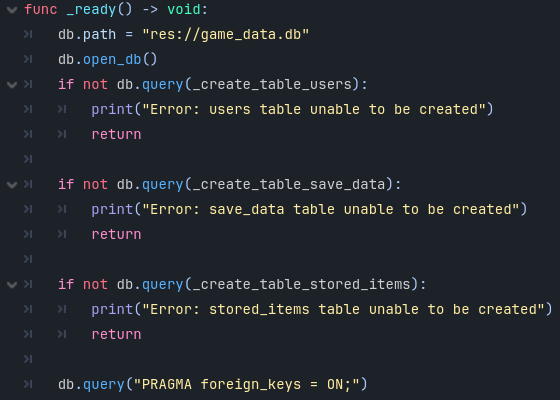
\includegraphics{images/development/database_ready.PNG}
                \caption{\_ready}
        \end{figure}
        In the database script db is declared using $SQLite.new()$ which is a wrapper class. I use the script to load the database and make sure all the necessary tables are present.\\
        I also made it so that the database is closed when the script exits the tree so as to make sure all the data is saved properly.\\
        \subsubsection{Hashing}
        \begin{figure}[H]
                \centering
                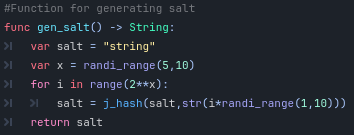
\includegraphics{images/development/gen_salt.PNG}
                \caption{gen\_salt}
        \end{figure}
        \begin{figure}[H]
                \centering
                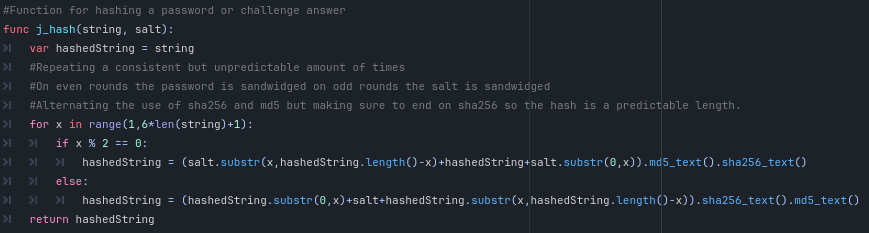
\includegraphics[width = \columnwidth]{images/development/hash.PNG}
                \caption{hash}
        \end{figure}
        \[\]
        The hash and gen\_salt functions implementation followed the pseudocode pretty faithfully apart from the fact I decided to not hash the number turned into a string as the salt doesnt have to be a certain length for the code to work. I also decided to times the number by a random integer to increase randomness and the number of possible salts.\\
        \subsubsection{Login Functions}
        \begin{figure}[H]
                \centering
                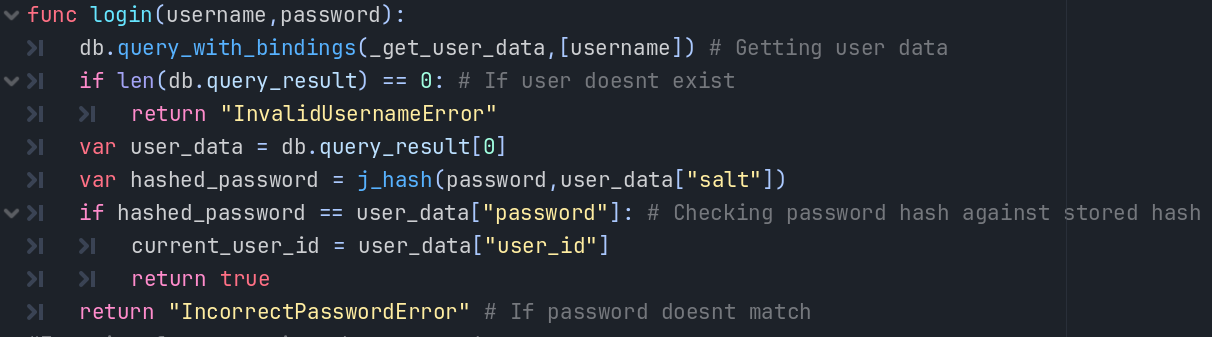
\includegraphics[width = \columnwidth]{images/development/login.PNG}
                \caption{login}
        \end{figure}
        This algorithm is a copy of the design algorithm just using godot's relevant functions instead. I further saved the current\_user\_id for ease of future queries.\\
        \begin{figure}[H]
                \centering
                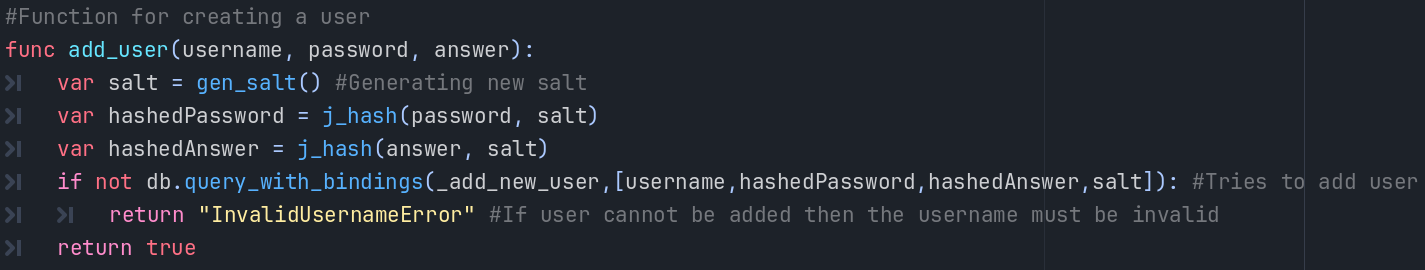
\includegraphics[width = \columnwidth]{images/development/add_user.PNG}
                \caption{add\_user}
        \end{figure}
        This algorithm is a copy of the design algorithm just using godot's relevant functions instead.\\
        \begin{figure}[H]
                \centering
                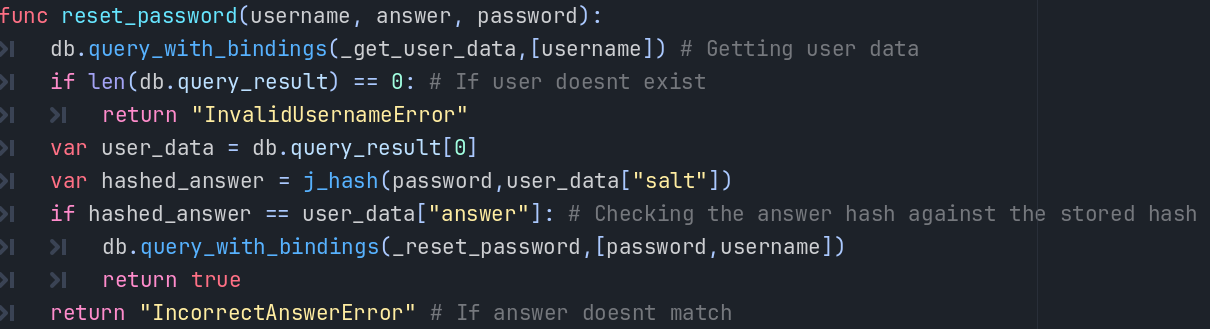
\includegraphics[width = \columnwidth]{images/development/reset_password.PNG}
                \caption{reset\_password}
        \end{figure}
        This algorithm is a copy of the design algorithm just using godot's relevant functions instead.\\
        \subsubsection{Testing}
        \begin{figure}[H]
                \centering
                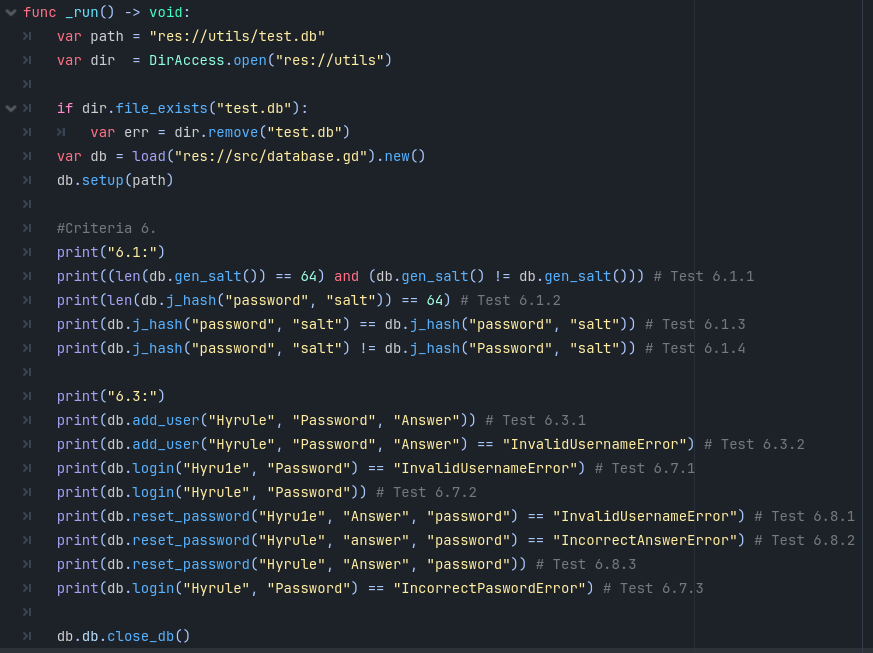
\includegraphics{images/development/test_database.PNG}
                \caption{test\_database.gd}
        \end{figure}
        \begin{tabular}{|c|c|c|c|c|}
                \hline
                Test \#&Function&Parameters&Expected Outcome&Actual Outcome\\
                \hline
                6.1.1&gen\_salt()&&\mr{2}{4cm}{random 256 bit hex string}&Success\\
                &&&&\\
                \hline
                6.1.2&hash()&"password", "salt"&\mr{2}{4cm}{random 256 bit hex string}&Success\\
                &&&&\\
                \hline
                6.1.3&hash()&"password", "salt"&\mr{2}{4cm}{the same random 256 bit hex string}&Success\\
                &&&&\\
                \hline
                6.1.2&hash()&"Password", "salt"&\mr{2}{4cm}{random 256 bit hex string different from before}&Success\\
                &&&&\\
                \hline
                6.3.1&add\_user()&"Hyrule", "Password", "Answer"&\mr{2}{4cm}{True}&Success\\
                &&&&\\
                \hline
                6.3.2&add\_user()&"Hyrule", "Password", "Answer"&\mr{2}{4cm}{"InvalidUsernameError" as a user already exists with that username}&Success\\
                &&&&\\
                &&&&\\
                \hline
                6.6.1&login()&"Hyru1e", "Password"&\mr{2}{4cm}{"InvalidUsernameError"}&Success\\
                &&&&\\
                \hline
                6.6.2&login()&"Hyrule", "Password"&\mr{2}{4cm}{True}&Success\\
                &&&&\\
                \hline
                6.7.1&reset\_password()&"Hyru1e", "Answer", "password&\mr{2}{4cm}{"InvalidUsernameError"}&Success\\
                &&&&\\
                \hline
                6.7.2&reset\_password()&"Hyrule", "answer", "password"&\mr{2}{4cm}{"IncorrectAnswerError"}&Success\\
                &&&&\\
                \hline
                6.7.3&reset\_password()&"Hyrule", "Answer", "password"&\mr{2}{4cm}{True}&Success\\
                &&&&\\
                \hline
                6.6.3&login()&"Hyrule", "Password"&\mr{2}{4cm}{"IncorrectPasswordError"}&Success\\
                &&&&\\
                \hline
        \end{tabular}
        \[\]
        Upon Testing I realised I needed a delete user function so that the user can be deleted.\\
        I designed a simple SQL query and created a function to delete users.\\
        \begin{figure}[H]
            \centering
            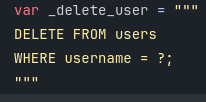
\includegraphics[width=0.3\columnwidth]{images/development/_delete_user.png}
            \caption{\_delete\_user}
        \end{figure}
        \begin{figure}[H]
            \centering
            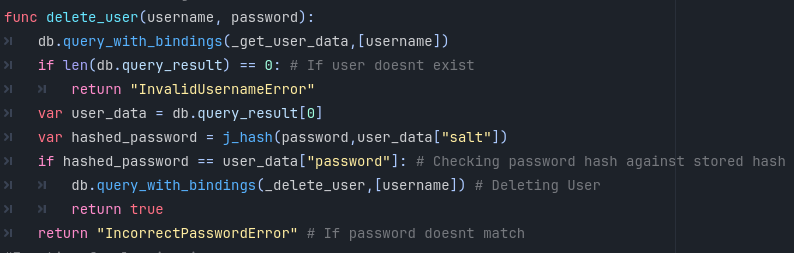
\includegraphics[width=0.7\columnwidth]{images/development/delete_user.png}
            \caption{delete\_user}
        \end{figure}
        \[\]
        \begin{tabular}{|c|c|c|c|c|}
                \hline
                Test \#&Function&Parameters&Expected Outcome&Actual Outcome\\
                \hline
                6.9.1&delete\_user()&"Hyrule", "Password"&\mr{1}{4cm}{IncorrectPasswordError}&Success\\
                \hline
                6.9.2&delete\_user()&"Hyrule", "password"&\mr{1}{4cm}{True}&Success\\
                \hline
                6.6.4&login()&"Hyrule", "password"&\mr{1}{4cm}{InvalidUsernameError}&Success\\
                \hline
                
        \end{tabular}
        \[\]
        \begin{figure}[H]
            \centering
            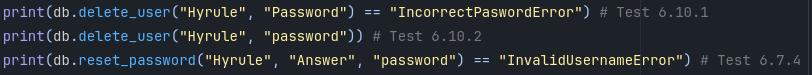
\includegraphics[width=0.8\columnwidth]{images/development/test_remove_user.png}
            \caption{Test Remove User}
        \end{figure}
        \[\]
        Upon Testing the remove functions in the database I have updated the table queries to add ON DELETE CASCADE so that if the user gets deleted all their saves get deleted.\\
        \subsection{Login System Development}
        I used godot's inbuilt label, button and line edit node's in order to construct my forms. To each form I added an extra label in order to display Errors to the user.\\
        I linked the buttons pressed signals to a script in order to determine what happens when the button is pressed and used variables to fetch and store the data from the line edit nodes.\\
        I used node2ds in order to create groups of the nodes for more organisation and I kept the form layout mostly the same without some of the fancier unnecesary design elements from the mockup forms.\\
        \newpage
        \subsubsection{Login Form}
        \begin{multicols}{2}
                \begin{figure}[H]
                        \centering
                        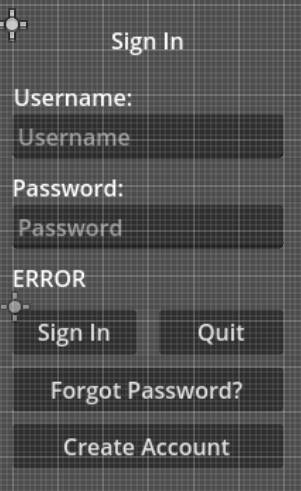
\includegraphics[width = 0.5\columnwidth]{images/development/LoginForm_layout.PNG}
                        \caption{Layout}
                \end{figure}
                \begin{figure}[H]
                        \centering
                        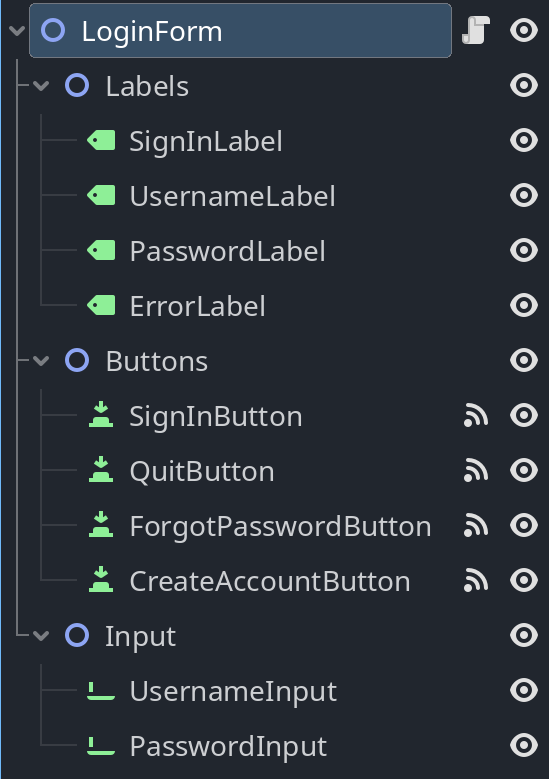
\includegraphics[width = 0.6\columnwidth]{images/development/LoginForm_structure.PNG}
                        \caption{Structure}
                \end{figure}
        \end{multicols}
        \[\]
        \begin{figure}[H]
              \centering
              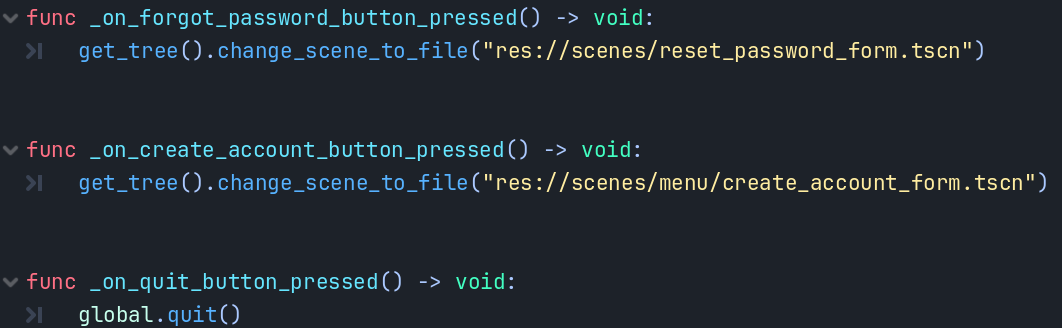
\includegraphics{images/development/LoginForm_buttons.PNG}  
              \caption{button\_pressed functions}
        \end{figure}
        These button functions are pretty simple as I only need to change scene or quit the game.\\
        \begin{figure}[H]
                \centering
                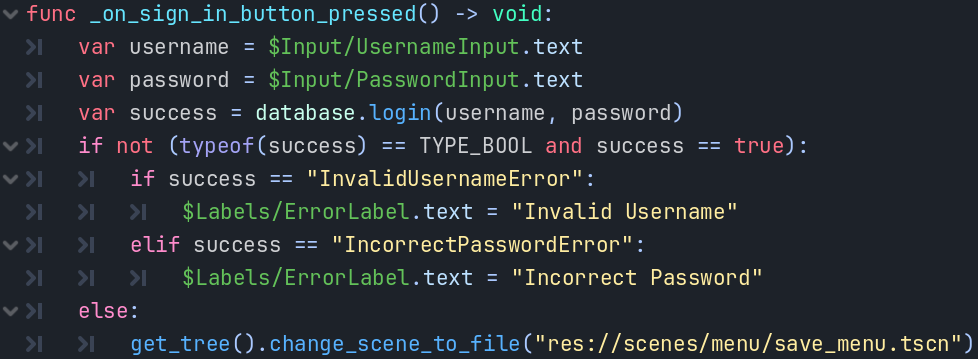
\includegraphics{images/development/_on_sign_in_button_pressed.PNG}
                \caption{\_on\_sign\_in\_button\_pressed}
        \end{figure}
        \[\]
        This is the function for when the sign in button is pressed it fetches the data and tries to login, displaying any errors it gets. If the login is successful theen it switches the scene to the save\_menu scene.\\
        \subsubsection{Reset Password Form}
        \begin{multicols}{2}
                \begin{figure}[H]
                        \centering
                        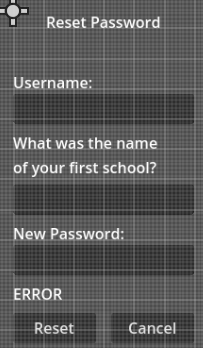
\includegraphics[width = 0.5\columnwidth]{images/development/ResetPasswordForm_layout.PNG}
                        \caption{Layout}
                \end{figure}
                \begin{figure}[H]
                        \centering
                        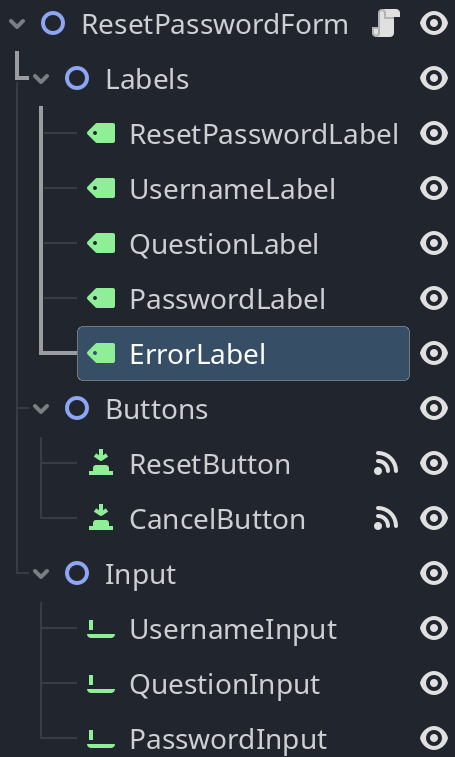
\includegraphics[width = 0.6\columnwidth]{images/development/ResetPasswordForm_structure.PNG}
                        \caption{Structure}
                \end{figure}
        \end{multicols}
        \[\]
        \begin{figure}[H]
              \centering
              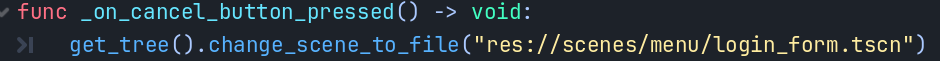
\includegraphics{images/development/ResetPasswordForm_cancel.PNG}
              \caption{\_on\_cancel\_button\_pressed}
        \end{figure}
        This button function is pretty simple as I only need to change scene back to the login form.\\
        \begin{figure}[H]
                \centering
                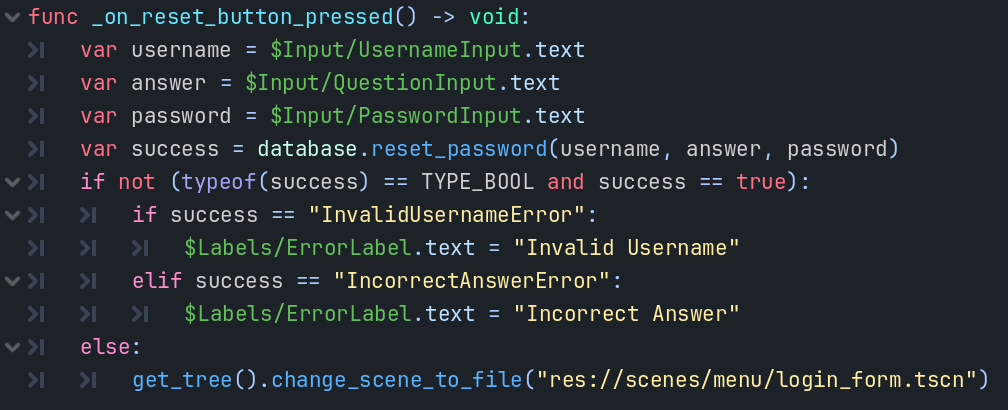
\includegraphics{images/development/ResetPasswordForm_reset.PNG}
                \caption{\_on\_reset\_password\_button\_pressed}
        \end{figure}
        \[\]
        This is the function for when the reset password button is pressed it fetches the data and tries to reset the password, displaying any errors it gets. If the reset is successful then it switches the scene to the login\_form scene.\\
        \subsubsection{Create Account Form}
        \begin{multicols}{2}
                \begin{figure}[H]
                        \centering
                        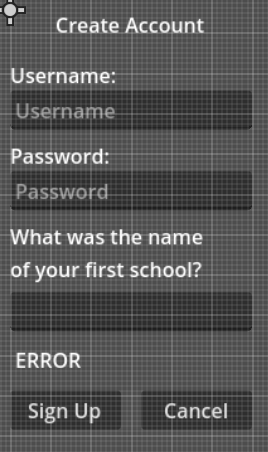
\includegraphics[width = 0.5\columnwidth]{images/development/CreateAccountForm_layout.PNG}
                        \caption{Layout}
                \end{figure}
                \begin{figure}[H]
                        \centering
                        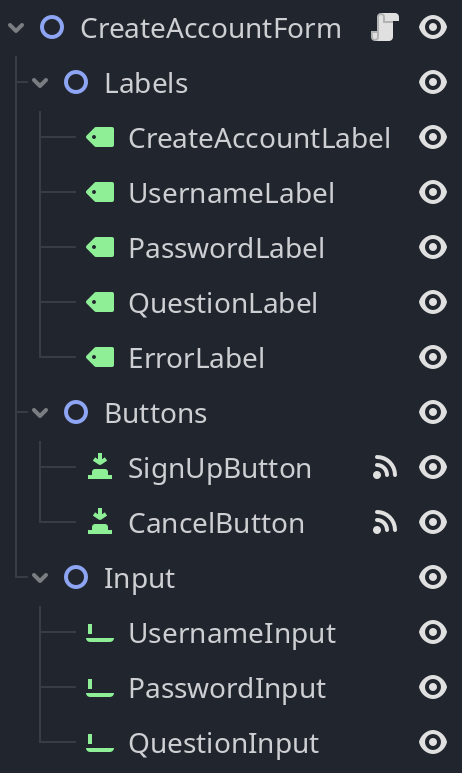
\includegraphics[width = 0.6\columnwidth]{images/development/CreateAccountForm_structure.PNG}
                        \caption{Structure}
                \end{figure}
        \end{multicols}
        \[\]
        \begin{figure}[H]
              \centering
              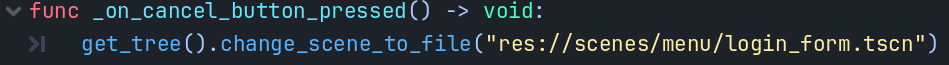
\includegraphics{images/development/CreateAccountForm_cancel.PNG}
              \caption{\_on\_cancel\_button\_pressed}
        \end{figure}
        This button function is pretty simple as I only need to change scene back to the login form.\\
        \begin{figure}[H]
                \centering
                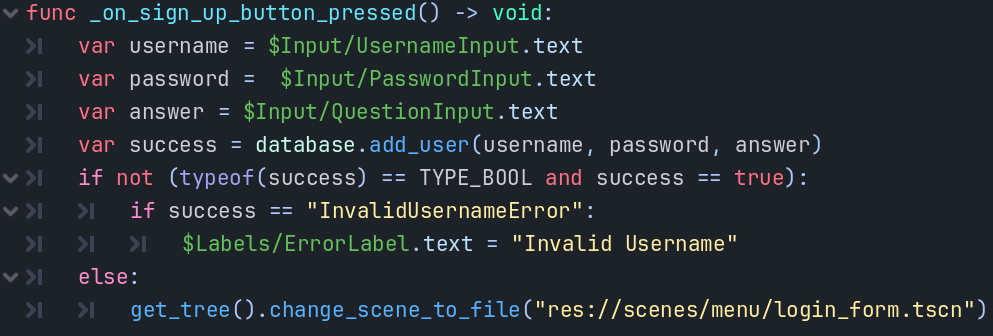
\includegraphics{images/development/CreateAccountForm_create.PNG}
                \caption{\_on\_reset\_password\_button\_pressed}
        \end{figure}
        \[\]
        This is the function for when the create account button is pressed it fetches the data and tries to create the account, displaying any errors it gets. If the reset is successful then it switches the scene to the login\_form scene.\\
        
        \newpage
        \subsection{Item Development}
        I will use resource scripts in order to implement the item classes and I will export the variables so that when I create new resources I can set the values.\\
        In order to export the armour\_type, body\_part, charm\_type, weapon\_type and damage\_type I will use an enum as it can only take one of the values in the list. This means the variables will take the form of an integer instead of a string.\\
        \subsubsection{Folder Structure}
        \begin{figure}[H]
                \centering
                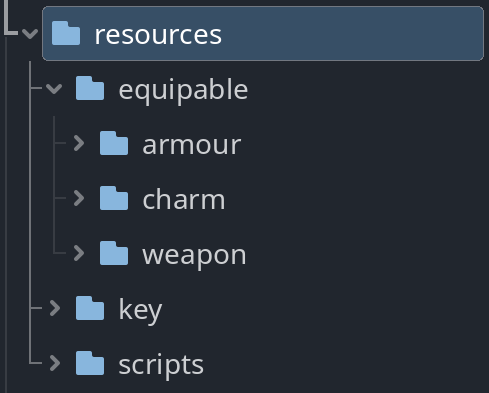
\includegraphics{images/development/Item_folder.PNG}
                \caption{Folder Structure}
        \end{figure}
        \[\]
        I added more folders in order to organise the items into their groups aswell as keeping the resource scripts in a scripts folder.\\
        \subsubsection{Item}
        \begin{multicols}{2}
                \begin{figure}[H]
                        \centering
                        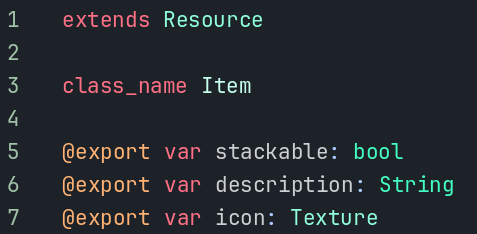
\includegraphics[width = 0.9\columnwidth]{images/development/Item_script.PNG}
                        \caption{Item Script}
                \end{figure}
                \begin{figure}[H]
                        \centering
                        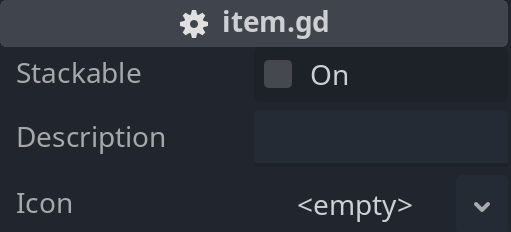
\includegraphics[width = 0.9\columnwidth]{images/development/Item_export.PNG}
                        \caption{Item Exports}
                \end{figure}
        \end{multicols}
        \[\]
        This shows the Item script and exported variables which I can set for each instance of that class including instances of classes that inherit from item.\\
        I chose to remove the item\_id as it seemed complicated to autoincrement it and enforce uniqueness and so I will store the file path in the item\_id column in the database instead of an integer and so I updated the create\_table\_stored\_items query in order to allow that.\\
        \newpage
        \subsubsection{Equipable}
        \begin{multicols}{2}
                \begin{figure}[H]
                        \centering
                        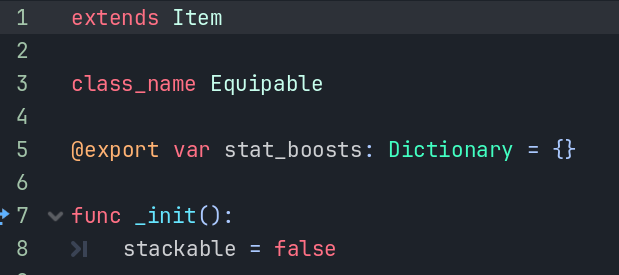
\includegraphics[width = 0.9\columnwidth]{images/development/Equipable_script.PNG}
                        \caption{Equipable Script}
                \end{figure}
                \begin{figure}[H]
                        \centering
                        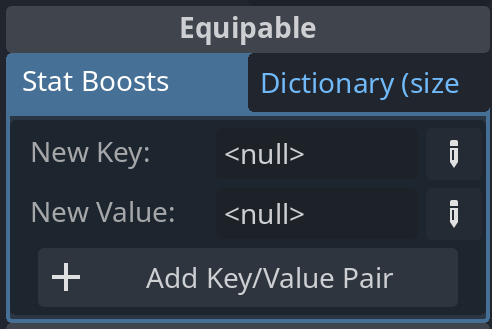
\includegraphics[width = 0.9\columnwidth]{images/development/Equipable_export.PNG}
                        \caption{Equipable Exports}
                \end{figure}
        \end{multicols}
        \[\]
        This shows the Equipable script and exported variables which I can set in any instance of this class or classes that inherit from it. I am using a dictionary to store stat boosts where the key is the stat and the value is the boost and these pairs can be added through the inspector. I set stackable to false by default as Equipable items will not be stackable.
        \subsubsection{Armour}
        \begin{multicols}{2}
                \begin{figure}[H]
                        \centering
                        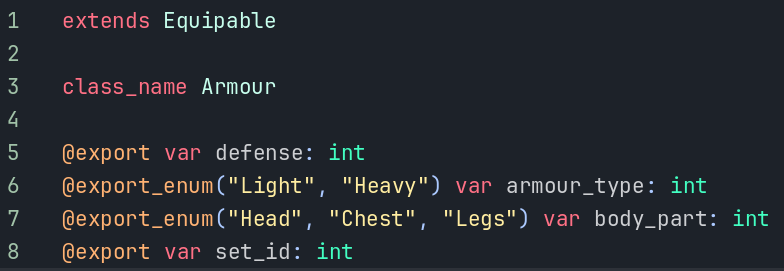
\includegraphics[width = \columnwidth]{images/development/Armour_script.PNG}
                        \caption{Armour Script}
                \end{figure}
                \begin{figure}[H]
                        \centering
                        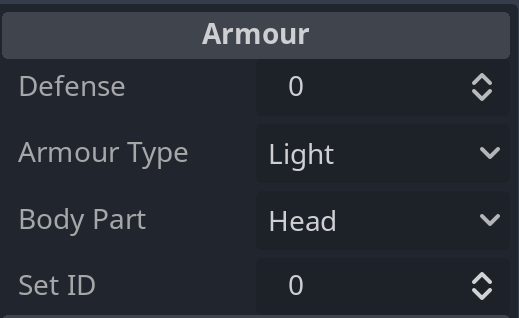
\includegraphics[width = 0.9\columnwidth]{images/development/Armour_export.PNG}
                        \caption{Armour Exports}
                \end{figure}
        \end{multicols}
        \[\]
        This shows the Armour script and exported variables which I can set in any instance. I used an enum to represent the types of armour and body parts which it can be equipped on.\\
        \subsubsection{Charm}
        \begin{multicols}{2}
                \begin{figure}[H]
                        \centering
                        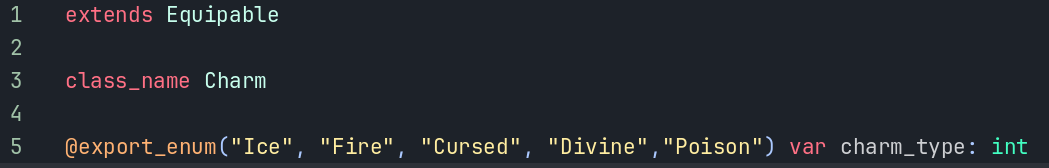
\includegraphics[width = \columnwidth]{images/development/Charm_script.PNG}
                        \caption{Charm Script}
                \end{figure}
                \begin{figure}[H]
                        \centering
                        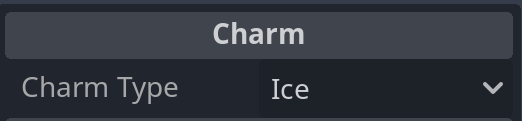
\includegraphics[width = 0.9\columnwidth]{images/development/Charm_export.PNG}
                        \caption{Charm Exports}
                \end{figure}
        \end{multicols}
        \[\]
        This shows the Charm script and exported variables which I can set in any instance. I used an enum to represent the different charm types as you can only have one of them.\\
        \subsubsection{Weapon}
        \begin{multicols}{2}
                \begin{figure}[H]
                        \centering
                        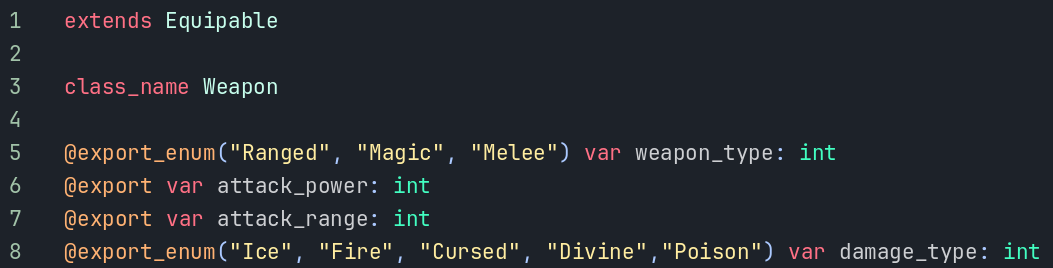
\includegraphics[width = \columnwidth]{images/development/Weapon_script.PNG}
                        \caption{Weapon Script}
                \end{figure}
                \begin{figure}[H]
                        \centering
                        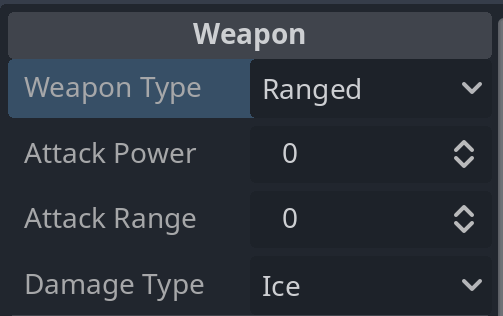
\includegraphics[width = 0.9\columnwidth]{images/development/Weapon_export.PNG}
                        \caption{Weapon Exports}
                \end{figure}
        \end{multicols}
        \[\]
        This shows the Weapon script and exported variables which I can set in any instance. I used an enum to represent the different weapon types and damage types so you can only select one
        \begin{figure}[H]
                \centering
                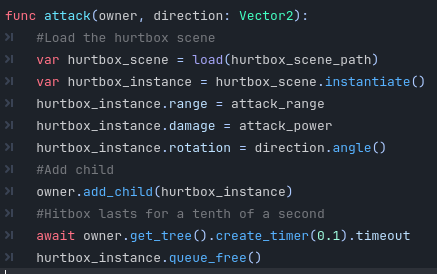
\includegraphics[width = 0.8\columnwidth]{images/development/Weapon_attack.PNG}
                \caption{Weapon attack() function}
        \end{figure}
        \noindent This shows the weapon attack script that I implemented I changed the name from hitbox to hurtbox as that is more accurate and I had to use a timer in order to sleep for an amount of time that the hitbox will last for.\\
        \subsubsection{Key}
        \begin{multicols}{2}
                \begin{figure}[H]
                        \centering
                        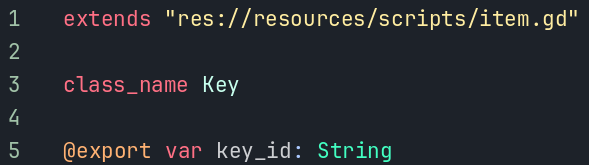
\includegraphics[width = \columnwidth]{images/development/Key_script.PNG}
                        \caption{Key Script}
                \end{figure}
                \begin{figure}[H]
                        \centering
                        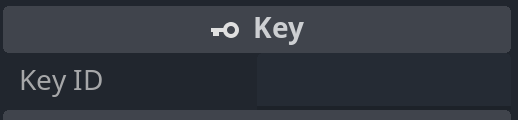
\includegraphics[width = 0.9\columnwidth]{images/development/Key_export.PNG}
                        \caption{Key Exports}
                \end{figure}
        \end{multicols}
        \[\]
        This shows the Key script and exported variables which I can set in any instance. The key ID will correspond to a door id and unlock that door.\\
        \subsubsection{Revision}
        Upon starting the inventory development I have decided to switch from enums to strings as the enums make it more complicated to access the string associated with the number.\\
        \subsection{Inventory Development}
        I used a seperate autoloaded script inventory.gd in order to implement the inventory functions.\\
        I added functions to the database script in order to utilise the current\_save\_id script variable so that I dont have to input the variable every time I want to run a save\_data or stored\_items query. The functions execute the query passing in the current\_save\_id and return the query result.\\
        \subsubsection{Add Item}
        \begin{figure}[H]
                \centering
                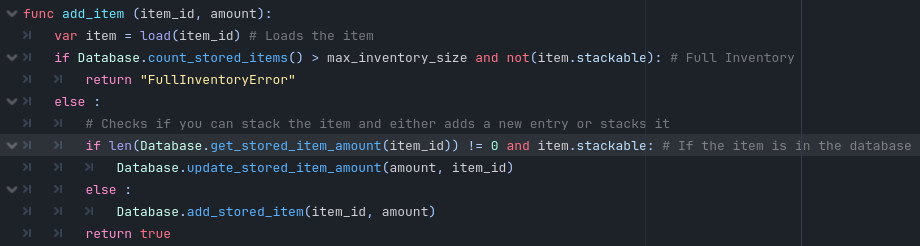
\includegraphics[width=0.8\columnwidth]{images/development/add_item.PNG}
                \caption{add\_item()}
        \end{figure}
        \[\]
        The add\_item function stayed mostly faithful to the pseudocode except I moved stuff arround for clarity.\\
        \subsubsection{Remove Item}
        \begin{figure}[H]
                \centering
                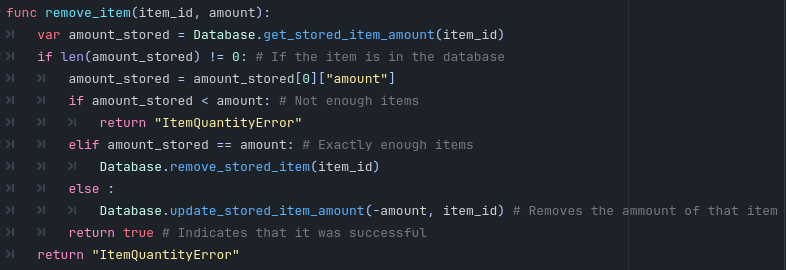
\includegraphics[width=0.8\columnwidth]{images/development/remove_item.PNG}
                \caption{remove\_item()}
        \end{figure}
        \[\]
        The remove\_item function is mostly the same as the pseudocode except I extracted some of the query data so I don't end up running repeat queries.\\
        \subsubsection{Unequip Item}
        \begin{figure}[H]
                \centering
                \includegraphics[width=0.8\columnwidth]{images/development/unequip_item.PNG}
                \caption{unequip\_item()}
        \end{figure}
        \[\]
        The unequip\_item function is again close to the pseudocode except I extracted repeat queries to a variable.\\
        \subsubsection{Equip Item}
        \begin{figure}[H]
                \centering
                \includegraphics[width=0.8\columnwidth]{images/development/equip_item.PNG}
                \caption{equip\_item()}
        \end{figure}
        In the equip item function I decided to simplify the proccess of deciding which charm slot as it was unnecesarily complex and I also added a check for if the inventory is full making sure to still accept it if equipping the item leaves just enough room in the inventory.\\
        \subsubsection{Testing}
        \begin{figure}[H]
                \centering
                \includegraphics[width=0.8\columnwidth]{images/development/test_inventory.PNG}
                \caption{test\_inventory()}
        \end{figure}
        \begin{tabular}{|c|c|c|c|c|}
                \hline
                Test \#&Function&Parameters&Expected Outcome&Actual Outcome\\
                \hline
                12.5.1&add\_item()&"test\_item.tres", 2&\mr{2}{5cm}{Adds test item to the stored\_items table.}&Success\\
                &&&&\\
                \hline
                12.5.2&add\_item()&"test\_item.tres", 3&\mr{2}{5cm}{As the item already exists it should add 3 to the amount.}&Success\\
                &&&&\\
                &&&&\\
                \hline
                12.5.3&add\_item()&"test\_weapon.tres", 1&\mr{2}{5cm}{As in the testing environment the max inventory size will be 1 and this should return "FullInventoryError"}&Fail\\
                &&&&\\
                &&&&\\
                &&&&\\
                \hline
                12.5.4&remove\_item()&"test\_item.tres", 2&\mr{2}{5cm}{As more than the amount of the item is in the inventory it should subtract 2.}&Success\\
                &&&&\\
                &&&&\\
                \hline
                12.5.5&remove\_item()&"test\_item.tres", 10&\mr{2}{5cm}{"ItemQuantityError" as there isnt enough of the item in the database}&Success\\
                &&&&\\
                &&&&\\
                \hline
                12.5.6&remove\_item()&"test\_item.tres", 3&\mr{2}{5cm}{As exactly the amount is in the database the item entry should get removed.}&Success\\
                &&&&\\
                &&&&\\
                \hline
                12.5.7&remove\_item()&"test\_item.tres", 2&\mr{2}{5cm}{"ItemQuantityError" as there isnt any of the item in the database}&Success\\
                &&&&\\
                &&&&\\
                \hline
                12.4.1&unequip\_item()&"head"&\mr{2}{5cm}{True and the head slot should remain as NULL}&Fail\\
                &&&&\\
                \hline
                12.4.2&equip\_item()&"test\_helmet.tres"&\mr{2}{5cm}{True and the head slot should become "test\_helmet.tres"}&Success\\
                &&&&\\
                \hline
                12.4.3&equip\_item()&"test\_helmet\_2.tres"&\mr{2}{5cm}{True and the head slot should become "test\_helmet.tres"}&Success\\
                &&&&\\
                \hline
                12.4.4&unequip\_item()&"head"&\mr{2}{5cm}{"FullInventoryError"}&Success\\
                &&&&\\
                \hline
                12.4.5&unequip\_item()&"head"&\mr{2}{5cm}{True as I will empty the inventory and the head should be NULL and the inventory should contain the helmet.}&Success\\
                &&&&\\
                &&&&\\
                &&&&\\
                \hline
        \end{tabular}
        \[\]
        The add\_item function failed to return "FullInventoryError" as it only checked if the item wasnt stackable not if it wasnt stackabled and already stored so I updated the script.\\
        \begin{figure}[H]
                \centering
                \includegraphics[width = 0.8\columnwidth]{images/development/add_item_2.PNG}
                \caption{add\_item() fixed}
        \end{figure}
        \[\]
        The remove\_item failed due to a syntax error with the SQL statement so I edited the get\_slot\_value function to query for all values and then look it up I also updated the set\_slot\_value function to query the slot using a match case rather than bindings.\\
        \begin{multicols}{2}
        \begin{figure}[H]
                \centering
                \includegraphics[width = 0.8\columnwidth]{images/development/get_slot_value.PNG}
                \caption{get\_slot\_value() fixed}
        \end{figure}
        \begin{figure}[H]
                \centering
                \includegraphics[width = 0.8\columnwidth]{images/development/set_slot_value.PNG}
                \caption{set\_slot\_value() fixed}
        \end{figure}
        \end{multicols}
        \[\]
        The unequip\_item function failed due to not checking if success is a boolean before comparing it so I amended it.\\
        \begin{figure}[H]
                \centering
                \includegraphics[width = 0.8\columnwidth]{images/development/unequip_item_2.PNG}
                \caption{unequip\_item() fixed}
        \end{figure}
        \[\]
        \textbf{Retesting:}\\
        \begin{tabular}{|c|c|c|c|c|}
                \hline
                Test \#&Function&Parameters&Expected Outcome&Actual Outcome\\
                \hline
                12.5.1&add\_item()&"test\_item.tres", 2&\mr{2}{5cm}{Adds test item to the stored\_items table.}&Success\\
                &&&&\\
                \hline
                12.5.2&add\_item()&"test\_item.tres", 3&\mr{2}{5cm}{As the item already exists it should add 3 to the amount.}&Success\\
                &&&&\\
                &&&&\\
                \hline
                12.5.3&add\_item()&"test\_weapon.tres", 1&\mr{2}{5cm}{As in the testing environment the max inventory size will be 1 and this should return "FullInventoryError"}&Success\\
                &&&&\\
                &&&&\\
                &&&&\\
                \hline
                12.5.4&remove\_item()&"test\_item.tres", 2&\mr{2}{5cm}{As more than the amount of the item is in the inventory it should subtract 2.}&Success\\
                &&&&\\
                &&&&\\
                \hline
                12.5.5&remove\_item()&"test\_item.tres", 10&\mr{2}{5cm}{"ItemQuantityError" as there isnt enough of the item in the database}&Success\\
                &&&&\\
                &&&&\\
                \hline
                12.5.6&remove\_item()&"test\_item.tres", 3&\mr{2}{5cm}{As exactly the amount is in the database the item entry should get removed.}&Success\\
                &&&&\\
                &&&&\\
                \hline
                12.5.7&remove\_item()&"test\_item.tres", 2&\mr{2}{5cm}{"ItemQuantityError" as there isnt any of the item in the database}&Success\\
                &&&&\\
                &&&&\\
                \hline
                12.4.1&unequip\_item()&"head"&\mr{2}{5cm}{True and the head slot should remain as NULL}&Success\\
                &&&&\\
                \hline
                12.4.2&equip\_item()&"test\_helmet.tres"&\mr{2}{5cm}{True and the head slot should become "test\_helmet.tres"}&Success\\
                &&&&\\
                \hline
                12.4.3&equip\_item()&"test\_helmet\_2.tres"&\mr{2}{5cm}{True and the head slot should become "test\_helmet.tres"}&Success\\
                &&&&\\
                \hline
                12.4.4&unequip\_item()&"head"&\mr{2}{5cm}{"FullInventoryError"}&Success\\
                &&&&\\
                \hline
                12.4.5&unequip\_item()&"head"&\mr{2}{5cm}{True as I will empty the inventory and the head should be NULL and the inventory should contain the helmet.}&Success\\
                &&&&\\
                &&&&\\
                &&&&\\
                \hline
        \end{tabular}
        Finally all my testing was a success.
        \subsection{Hurtbox Development}
        \subsubsection{Layout}
        \begin{figure}[H]
                \centering
                \includegraphics{images/development/HurtBox.PNG}
                \caption{HurtBox Layout}
        \end{figure}
        I made the hurtbox like this as the center of the area2d node (the cross) can rotate allowing the actual collisionshape to rotate around the player depending on the direction of attack.\\
        \subsubsection{Script}
        \begin{figure}[H]
                \centering
                \includegraphics{images/development/HurtBox_Script.PNG}
                \caption{Hurtbox Script}
        \end{figure}
        I changed the script from using the ready function to running every time a body enters the hurtbox as it allows the hurtbox to work for the duration of its existence rather than just at the start. Other than that the script is the same.\\
        \subsection{Player Development}
        \subsubsection{Layout and Structure}
        \begin{multicols}{2}
                \begin{figure}[H]
                        \centering
                        \includegraphics{images/development/Player_layout.png}
                        \caption{Layout}
                \end{figure}
                \begin{figure}[H]
                        \centering
                        \includegraphics[width = 0.8\columnwidth]{images/development/Player_structure.png}
                        \caption{Structure}
                \end{figure}
        \end{multicols}
        \noindent The structure is the same as was described in the class diagram and the layout is as such so that the player can interact with walls and enemy hits can register it.\\
        \subsubsection{\_physics\_proccess(delta):}
        \begin{figure}[H]
                \centering
                \includegraphics[width = 0.8\columnwidth]{images/development/Player_physics_process().PNG}
                \caption{\_physics\_process():}
        \end{figure}
        \noindent I decided to add an animating flag for use in this script that will be flagged when animations that cannnot be interrupted are playing (e.g. attacks) so that the player will not move or switch animations during that. Other than that the function is the same as the designed function with a slightly different method of getting direction.\\
        \subsubsection{Player Animation}
        \begin{figure}[H]
                \centering
                \includegraphics[width = 0.8\columnwidth]{images/development/Animations.PNG}
                \caption{Animations}
        \end{figure}
        I added the animation frames into seperate animations in the Player's animationPlayer naming them such that the different directional animation names can be got using the get\_animation() function.\\
        \begin{figure}[H]
                \centering
                \includegraphics[width = 0.5\columnwidth]{images/development/Player_get_anim.PNG}
                \caption{get\_animation():}
        \end{figure}
        \subsection{Dummy Development}
        As part of my developmental testing I deciced to create a simple dummy to test weapons on. The dummy consists of a StaticBody2D with a CollisionShape2D and a Sprite2D it also has a simple script for taking damage which I have set to print damage type and damage to the console.\\
        \begin{multicols}{3}
                \begin{figure}[H]
                        \centering
                        \includegraphics[width = 0.9\columnwidth]{images/development/Dummy_layout.PNG}
                        \caption{Layout}
                \end{figure}
                \begin{figure}[H]
                        \centering
                        \includegraphics[width = 0.9\columnwidth]{images/development/Dummy_structure.PNG}
                        \caption{Structure}
                \end{figure}
                \begin{figure}[H]
                        \centering
                        \includegraphics[width = 0.9\columnwidth]{images/development/Dummy_script.PNG}
                        \caption{Script}
                \end{figure}
        \end{multicols}
        \subsection{Dungeon Environment Development}
        \subsubsection{Door}
        \begin{multicols}{2}
                \begin{figure}[H]
                        \centering
                        \includegraphics[width = 0.9\columnwidth]{images/development/Door_layout.PNG}
                        \caption{Layout}
                \end{figure}
                \begin{figure}[H]
                        \centering
                        \includegraphics[width = 0.9\columnwidth]{images/development/Door_structure.PNG}
                        \caption{Structure}
                \end{figure}   
        \end{multicols}
        \noindent The layout and structure of the door is as shown above, mostly the same as was designed making sure to get the area2d infront of the door for opening.\\
        \begin{figure}[H]
                \centering
                \includegraphics[width = 0.9\columnwidth]{images/development/Door_script.PNG}
                \caption{Script}
        \end{figure}
        \noindent I added a variable that detemines wether or not the door is locked aswell as looping through the overlapping bodies instead of checking if it overlaps a certain body as that was easier to implement.\\
        \subsubsection{Chest}
        \begin{multicols}{2}
                \begin{figure}[H]
                        \centering
                        \includegraphics[width = 0.9\columnwidth]{images/development/Chest_layout.PNG}
                        \caption{Layout}
                \end{figure}
                \begin{figure}[H]
                        \centering
                        \includegraphics[width = 0.9\columnwidth]{images/development/Chest_structure.PNG}
                        \caption{Structure}
                \end{figure}   
        \end{multicols}
        \noindent The layout and structure of the chest are mostly the same as was designed with the detection area being a circle around the chest.
        \begin{figure}[H]
                \centering
                \includegraphics[width = 0.9\columnwidth]{images/development/Chest_script.PNG}
                \caption{Script}
        \end{figure}
        \noindent The chest script is has a couple changes from the design, the addition of a locked flag aswell as making the item list a script variable so that it can be accessed from the input function and constructing the list without the use of pythonic list comprehension. I also switched from directly seeing if the player body overlaps to looping through overlapping bodies again as this wasy easier to implement and works the same.\\
        \subsection{Enemy Development}
        \subsubsection{Layout and Structure}
        \begin{multicols}{2}
                \begin{figure}[H]
                        \centering
                        \includegraphics[width = 0.9\columnwidth]{images/development/Enemy_layout.PNG}
                        \caption{Layout}
                \end{figure}
                \begin{figure}[H]
                        \centering
                        \includegraphics[width = 0.9\columnwidth]{images/development/Enemy_structure.PNG}
                        \caption{Structure}
                \end{figure}   
        \end{multicols}
        The layout and structure are as shown above with all the relevant timer nodes, the larger collision shape is the area2D for detecting the player whereas the smaller one handles physics collisons. The NavigationAgent2D handles the navigation and the AnimatedSprite2D handles animation.\\
        \subsubsection{General Script}
        \begin{multicols}{2}
                \begin{figure}[H]
                        \centering
                        \includegraphics[width = 0.8\columnwidth]{images/development/Enemy_script.PNG}
                        \caption{General Script and Variables}
                \end{figure}
                \begin{figure}[H]
                        \centering
                        \includegraphics[width = 0.9\columnwidth]{images/development/Enemy_ready.PNG}
                        \caption{\_ready():}
                \end{figure}   
                \begin{figure}[H]
                        \centering
                        \includegraphics[width = 0.9\columnwidth]{images/development/Enemy_timer_timeouts.PNG}
                        \caption{timer\_timeouts}
                \end{figure}
        \end{multicols}
        \subsubsection{\_physics\_process(delta):}
        \subsubsection{take\_damage(damage, damage\_type):}
        \subsubsection{Animation}
\newpage
\section{References}
\begin{tabular}{|c|c|c|c|c|c|}
        \hline
        REF$\#$ &Date&Topic/Abstract&Type&URL or BOOK reference&How I used this\\
        \hline
        1&1/6/24&\mr{2}{3cm}{Research/ Existing Solutions}&\mr{2}{2cm}{video games store, online}& \mr{2}{4cm}{\href{https://store.steampowered.com/app/113200/The_Binding_of_Isaac}{Steam (The Binding of Isaac)}}&\mr{2}{3cm}{One of the exisiting solutions I researched.}\\
        &&&&&\\
        &&&&&\\
        \hline
        2&15/6/24&\mr{2}{3cm}{Research/ Existing Solutions}&\mr{2}{2cm}{video games store, online}& \mr{2}{4cm}{\href{https://store.steampowered.com/app/588650/Dead_Cells}{Steam (Dead Cells)}}&\mr{2}{3cm}{One of the existing solutions I researched}\\
        &&&&&\\
        &&&&&\\
        \hline
        3&15/6/24&\mr{2}{3cm}{Research/ Existing Solutions}&\mr{2}{2cm}{youtube video, online}&\mr{2}{4cm}{\href{https://www.youtube.com/watch?v=tyMrRW-Li_I}{Youtube (Motion Twin)}}&\mr{2}{3cm}{A dev log for an existing solution.}\\
        &&&&&\\
        \hline
        4&15/6/24&\mr{2}{3cm}{Research/ Existing Solutions}&\mr{2}{2cm}{blog, online}&\mr{2}{4cm}{\href{https://robertheaton.com/2018/12/17/wavefunction-collapse-algorithm/}{robertheaton.com}}&\mr{2}{3cm}{An existing algorithm I researched.}\\
        &&&&&\\
        &&&&&\\
        \hline
        5&25/11/24&\mr{3}{3cm}{Research/ Exisiting Solutions}&\mr{2}{2cm}{video games store, online}&\mr{2}{4cm}{\href{https://store.nintendo.co\\.uk/en/the-legend-of-zelda-breath-of-the-wild-70010000000023}{Nintendo Store (Breath of The Wild)}}&\mr{2}{3cm}{One of the existing solutions I researched}\\
        &&&&&\\
        &&&&&\\
        \hline
        6&04/03/25&\mr{3}{3cm}{Design/ Enemy Design}&\mr{2}{2cm}{Game Engine Documentation, online}&\mr{2}{4cm}{\href{https://docs.godotengine.org/en/stable/tutorials/navigation/navigation_introduction_2d.html}{Godot Docs (2D navigation)}}&\mr{2}{3cm}{The documentation for godot's navigation nodes in 2D}\\
        &&&&&\\
        &&&&&\\
        &&&&&\\
        \hline
\end{tabular}
\end{document}